% =====================================================================
%  ijece-en.tex - Versi PADAT (maks ~14 halaman) dari ijece.tex.
%  Substansi, tabel, angka, gambar (16), dan 46 referensi dipertahankan;
%  yang dipangkas hanya verbositas narasi dan ukuran gambar.
% =====================================================================
\documentclass{iaesarticle}

\setlength{\headsep}{0.15in}
\usepackage{amsmath, amsfonts, amssymb, float, fancyhdr}
\usepackage[figuresright]{rotating}
\usepackage{authblk, graphicx, indentfirst, lastpage, lipsum}
\usepackage{pifont}
\renewcommand{\Authsep}{, }
\renewcommand{\Authand}{, }
\renewcommand{\Authands}{, }
\setlength{\affilsep}{0cm}
\renewcommand\Authfont{\normalsize}
\renewcommand\Affilfont{\fontsize{8}{10}\mdseries}
\makeatletter
\renewcommand{\@biblabel}[1]{[#1]\hfill}
\renewcommand\AB@authnote[1]{\textsuperscript{\normalfont\bfseries#1}}
\makeatother
\usepackage[font=normalsize]{subfig, caption}
\usepackage{epstopdf}
\usepackage[left=3cm, right=2.5cm, top=2.5cm, bottom=2.5cm, includehead, includefoot]{geometry}
\usepackage[justification=centering]{caption}
\captionsetup{labelsep=period}
\usepackage{titlesec}
\usepackage[table]{xcolor}
\titleformat{\section}
{\normalfont\normalsize\bfseries\uppercase}{\thesection}{1.7em}{}
\titleformat{\subsection}
{\normalfont\normalsize\bfseries}{\thesubsection}{.95em}{}
\titleformat{\subsubsection}
{\bfseries}{\thesubsubsection}{.2em}{}
\titlespacing*{\section}{0cm}{0.7cm}{0cm}
\usepackage{enumitem}
\usepackage[numbers,sort&compress]{natbib}
\usepackage{ragged2e}
\usepackage{hyperref,graphicx}
\usepackage{multirow}
\usepackage{tabularx}
\usepackage{booktabs}
\usepackage{fleqn}
\usepackage{tikz}
\usetikzlibrary{arrows.meta, positioning, shapes.geometric}

\CopyrightLine[]{}{\textit{This is an open access article under the \textcolor{blue}{\underline{CC BY-SA}} license.}
\vspace{.5em}}

\author[1]{\bfseries Hero Yudo Martono}
\author[2]{\bfseries Nafisah Rahmadani Harahap}
\author[3]{\bfseries Iwan Syarif}
\author[4]{\bfseries Ferry Astika Saputra}
\affil[1,2,3,4]{Department of Informatics Engineering, Politeknik Elektronika Negeri Surabaya, Surabaya, Indonesia}

\title{Design of a cloud backup system based on multi-compression algorithms for ransomware attack mitigation}
\shorttitle{Design of a cloud backup system based on multi-compression algorithms ... (Martono)}

\begin{document}
\setcounter{page}{1}
\setlength{\parindent}{1.27cm}
\pagestyle{fancy}
\fancyhfoffset{0cm}

\journalname{International Journal of Electrical and Computer Engineering (IJECE)}
\journalshortname{Int J Elec \& Comp Eng}
\journalhomepage{http://ijece.iaescore.com}
\vol{99}
\no{1}
\months{Month}
\years{2099}
\issn{2088-8708}
\DOI{10.11591}
\pagefirst{1}
\pagelast{1x}
\IDpaper{42551}

\maketitle

\hrule
\vspace{.1em}
\hrule
\vspace{.5em}
\noindent
\parbox[t][][s]{0.315\textwidth}{%
\textbf{Article Info}
\vspace{.5em}
\hrule
\vspace{.5em}
\begin{history}
\vspace{.5em}
Received month dd, yyyy

Revised month dd, yyyy

Accepted month dd, yyyy

\vspace{.7em}
\end{history}
\vspace{.5em}
\hrule
\vspace{.5em}
\begin{keyword}
\vspace{.5em}
Air gapped backup \sep
Anomaly detection \sep
Cloud backup and restore \sep
Lossless compression \sep
Ransomware resilience
\vspace{.5em}
\end{keyword}
\vspace{\fill}
}
\parbox{0.020\textwidth}{\hspace{0.5em}}
\parbox[t][][s]{0.65\textwidth}{%
\begin{abstract}
\vspace{.3em}
Ransomware threatens the availability and integrity of data in cloud storage, and conventional backups remain vulnerable when the repository is directly reachable from the primary system, while single-algorithm compression is inefficient for heterogeneous file types. This study proposes a cloud backup system that integrates a logical \textit{air-gapped} mechanism with adaptive multi-algorithm \textit{lossless} compression to improve resilience and storage efficiency. The system uses SHA-256 \textit{hash} verification, metadata analysis, and file-structure inspection to distinguish legitimate backup encryption from ransomware-induced modification. Evaluation was performed in a controlled manner using a simulated attack model---without executing real \textit{malware}---on a limited synthetic \textit{dataset} of 43 files of varying types and sizes, under both normal and attacked conditions, and replicated on AWS EC2 (Windows and Linux). For low-entropy text files, compression reduced storage by up to 89.5\% (logs) and 81.1\% (CSV), whereas already-compressed files (JPG, XLSX) approached 0\%, consistent with information theory. The adaptive strategy completed the whole dataset about $21\times$ faster than static Gzip while still saving 43.3\% of storage. The system recovered all 43 affected files without error and, under the controlled conditions, achieved 0\% false positive rate (FPR) and 0\% false negative rate (FNR). Overall, the proposed approach strengthens the security, resilience, and storage efficiency of cloud backup against ransomware.
\end{abstract}
}
\parbox[l]{\textwidth}{%
\rule{0.275\textwidth}{0.5pt} \hspace{0.5cm} \hrulefill
\\
\emph{\textbf{Corresponding Author:}}
\vspace{.5em}\\
Hero Yudo Martono\\
Department of Informatics Engineering, Politeknik Elektronika Negeri Surabaya\\
Surabaya, Indonesia\\
Email: hero@pens.ac.id
}
\vspace{.5em}
\hrule
\vspace{.1em}
\hrule

\section{Introduction}
\label{sec:introduction}
Over the past decade, digital transformation---particularly in finance---has driven an exponential growth of data (transaction records, logs, user data, financial reports, and audit documents) that must be archived securely and efficiently for operational, audit, and regulatory purposes \cite{1}, \cite{2}, \cite{3}, \cite{4}, \cite{5}. A single financial institution may generate hundreds of gigabytes to terabytes daily, demanding storage that is secure, economical, and backed by mechanisms that keep data available and intact.

Among cyber threats, ransomware is the most alarming: it encrypts victims' data and demands a ransom, and modern variants also target network-connected backup infrastructure \cite{5}, \cite{6}, \cite{7}, \cite{8}. Once backups are infected, recovery becomes impossible, causing operational, financial, and reputational damage \cite{9}; Sophos reports that about 43\% of devices in financial organizations were affected in 2024. Conventional always-connected backups are therefore inadequate. A proven countermeasure is the \textit{air-gapped} architecture, which isolates backup storage---physically or logically---from the primary network \cite{10}. Because a fully physical \textit{air-gap} is costly and complex for small and medium organizations, this study adopts a \textbf{logical air-gap} using controlled \textit{mounting} and isolated media, prioritizing affordability, ease of deployment, and compatibility with common cloud infrastructures.

The scale of the threat has surged: a survey of 50+ articles (2020--2025) records global losses exceeding USD~30 billion in 2023 ($\approx$900\% rise from 2015), 493 million attacks in 2022, an average ransom of USD~2.73 million in 2024, and 21 days average disruption \cite{41}. Ransomware has entered the \textit{data-exfiltration} era with \textit{double}/\textit{triple extortion} and a \textit{Ransomware-as-a-Service} (RaaS) model, while academic research lags behind real attack patterns \cite{23}, \cite{26}, \cite{40}, \cite{33}. Preventing infection alone is no longer sufficient \cite{42}, \cite{46}. The literature organizes defenses via the \textit{Detection--Avoidance--Mitigation} (DAM) framework \cite{42}; within it, this study occupies the \textbf{mitigation and recovery} stage, ensuring data remain recoverable even when early detection fails, rather than competing on \textit{machine-learning} detection accuracy.

Storage efficiency is equally important. For rarely accessed data, organizations use cold cloud storage \cite{11}, where \textit{lossless} compression trims cost without harming integrity \cite{12}, \cite{13}. However, prior work generally treats backup security, ransomware mitigation, or compression separately \cite{14}, \cite{15}, and mostly relies on a single static algorithm despite the non-uniform compression behavior of different file types \cite{16}, \cite{17}.

The link between compression and security stems from \textit{entropy}. Shannon's theory sets the \textit{lossless} limit as $H(X) = -\sum_{i} p(x_i)\log_2 p(x_i)$: low-entropy files (CSV, logs) are highly redundant and compress well, whereas high-entropy files (encrypted or already-compressed JPG) are near-random and barely compress. Two consequences follow: (i) the algorithm should adapt to file entropy/type, and (ii) a sudden entropy spike can signal illegitimate encryption---though \textit{Format-Preserving Encryption} (FPE) can evade entropy-based detection by preserving structure. This defines our \textit{research gap}: no single framework yet unites (a) adaptive compression by file characteristics, (b) ransomware-resilient backup isolation, and (c) integrity verification based on \textit{hash} and metadata rather than entropy alone.

Accordingly, this study proposes an integrated cloud backup system combining an \textit{air-gapped} architecture with an adaptive framework that dynamically selects among five \textit{lossless} algorithms (Gzip, Zstandard, Brotli, LZ4, Snappy) via rule-based selection on file size and type. It further embeds multi-indicator anomaly detection---SHA-256 \textit{hash} analysis, metadata validation, and file-structure inspection---to separate ransomware encryption from legitimate AES-256 encryption. The contribution is thus an integrated approach that simultaneously addresses ransomware resilience, backup isolation, adaptive compression efficiency, and integrity verification within one framework for cloud-based financial data infrastructures \cite{18}, \cite{19}, \cite{20}.

\section{Related Work}
\label{sec:related_work}
Prior studies on cloud backup, compression, and ransomware mitigation mostly address a single aspect in isolation and rarely contrast \textit{air-gapped} with conventional connected backups. Table~\ref{tab:related_work} compares representative studies with the proposed system.

\begin{table}[H]
\centering
\fontsize{8pt}{10pt}\selectfont
\caption{Related work}
\label{tab:related_work}
\begin{tabularx}{\textwidth}{@{}c p{2.2cm} X X X X@{}}
\hline
\textbf{No} & \textbf{Study} & \textbf{Research Focus} & \textbf{Methods} & \textbf{Limitations} & \textbf{Contribution of this study} \\
\hline
1 & Smith and Lee, 2023 & Compression algorithm evaluation & Gzip, Zstd, Brotli, LZ4, Snappy & No backup security & Integrates compression with backup \\
2 & Kumar and Patel, 2024 & Compression in cloud e-commerce & Brotli, Snappy, Gzip & Only data-transfer performance & Applied within backup for storage efficiency \\
3 & Novak et al., 2021 & Backup for ransomware mitigation & Hybrid compression + air-gapped & Limited to finance sector & Cloud backup with anomaly detection \\
4 & Kumar and Patel, 2022 & Cloud backup vs ransomware & Zstd, LZ4, Gzip & No multi-algorithm comparison & Evaluates multiple algorithms \\
5 & Sahu and Panda, 2025 & Compression study & Snappy, Gzip, BZIP2 & Limited efficiency analysis & Integrates efficiency and security \\
6 & NIST (2024) guideline & Secure offline backup & Physical/logical air-gapped & No storage optimization/compression & Combines air-gap + adaptive compression + detection \\
\hline
\end{tabularx}
\end{table}

Smith and Lee evaluated compression algorithms without ransomware protection; Kumar and Patel optimized storage but lacked anomaly detection and automated recovery; Novak et al. introduced \textit{air-gapped} backup but did not comprehensively evaluate storage efficiency. The novelty here is integrating \textit{air-gapped} protection, adaptive multi-algorithm \textit{lossless} compression, and \textit{hash}/metadata anomaly detection in one architecture, improving resilience, efficiency, automated recovery, and practical deployment.

To position this work against the ransomware-detection mainstream: classical ML achieves high accuracy with feature selection \cite{31}, deep models (CNN, LSTM, CNN--LSTM) reach 96--99\% on balanced \textit{datasets} \cite{30}, hardware-assisted detection leverages AutoML \cite{34}, and real-time AES-NI monitoring can halt attacks after 10--15 files \cite{32}. Yet these face outdated \textit{datasets}, cross-platform difficulty, and evasion such as FPE \cite{43}, \textit{fileless}, and \textit{Living-off-the-Land} \cite{35}. This study \textbf{does not compete on detection accuracy}; it strengthens the \textit{mitigation/recovery} layer, aligned with backup-strategy work (3-2-1, \textit{immutable}/WORM, \textit{air-gapped}) reporting high recovery without ransom \cite{44} and structured incident response \cite{45}. It is therefore complementary to ML detectors: when detection fails, integrity checks and isolated recovery guarantee availability. Table~\ref{tab:airgap_comparison} contrasts \textit{air-gapped} and non-\textit{air-gapped} backup.

\begin{table}[H]
\centering
\fontsize{8pt}{10pt}\selectfont
\caption{Conceptual comparison of air-gapped and non air-gapped backup systems}
\label{tab:airgap_comparison}
\begin{tabularx}{\textwidth}{@{}p{3.2cm} X X@{}}
\hline
\textbf{Aspect} & \textbf{Air-Gapped Backup} & \textbf{Non Air-Gapped Backup} \\
\hline
Network connectivity & Isolated (physical or logical) & Connected to primary system \\
Ransomware resistance & High & Low \\
Risk of backup infection & Minimal & Potentially compromised \\
Data integrity & Preserved & Uncertain / failed \\
Recovery capability & Reliable & Uncertain / failed \\
Security level & Very high & Moderate \\
Compression strategy & Adaptive multi-algorithm & Single static compression \\
Storage efficiency & Up to 70--80\% reduction & Moderate \\
\hline
\end{tabularx}
\end{table}

In practice, many small and medium organizations still rely on connected cloud backups with single-algorithm compression, which remain vulnerable because repositories are directly reachable from compromised systems. The proposed system adds logical \textit{air-gapped} isolation, automated integrity verification, adaptive compression, and ransomware-aware recovery, achieving up to 70--80\% storage reduction for large structured data while maintaining 100\% recovery in simulation.

\section{Method}
\label{sec:method}
This study uses a quantitative experimental design to evaluate a cloud backup system integrating multiple \textit{lossless} compression algorithms \cite{22}, \cite{24}, \cite{25}. Each algorithm is tested independently, evaluating storage efficiency, processing time, and resilience to simulated ransomware. The system adopts a hybrid \textit{air-gapped} architecture combining offline local and cloud storage \cite{21}, \cite{27}, in an environment resembling real financial information systems \cite{28}, \cite{29}.

\subsection{System architecture}
The architecture has three logical layers. The \emph{application layer} manages upload, backup, and restore; each file undergoes SHA-256 \textit{hash} computation, metadata extraction, and structure analysis to form an integrity baseline distinguishing legitimate modification from malicious alteration. The \emph{protection and compression layer} inspects metadata, then \textbf{compresses first} using one of five algorithms and \textbf{only then encrypts} with AES-256. This \textit{compress-then-encrypt} order is essential: encrypted data has high entropy and cannot be compressed effectively, so compressing \textit{plaintext} first yields genuine savings before confidentiality is applied \cite{9}. The \emph{storage and detection layer} stores encrypted-compressed files in an \textit{air-gapped} environment and synchronizes to cloud storage (Google Drive API or Amazon S3) for redundancy; on detecting ransomware, it auto-recovers from \textit{air-gapped} storage via decryption and decompression. Figure~\ref{fig:architecture} shows the flow.

\begin{figure}[H]
\centering
\resizebox{0.9\textwidth}{!}{%
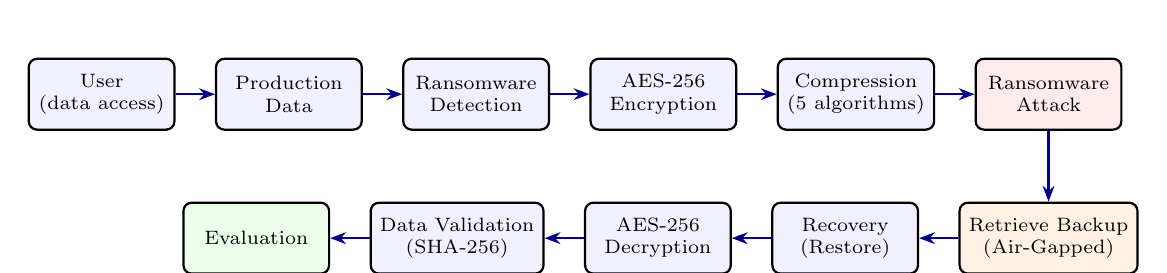
\begin{tikzpicture}[
    font=\scriptsize,
    node distance=0.4cm and 0.5cm,
    stage/.style={draw, rounded corners=3pt, minimum width=1.85cm, minimum height=0.9cm,
                  align=center, fill=blue!6, thick},
    ar/.style={-{Stealth[length=2mm]}, thick, blue!55!black}
]
\node[stage] (user)  {User\\(data access)};
\node[stage, right=of user] (prod)  {Production\\Data};
\node[stage, right=of prod] (det)   {Ransomware\\Detection};
\node[stage, right=of det]  (enc)   {AES-256\\Encryption};
\node[stage, right=of enc]  (comp)  {Compression\\(5 algorithms)};
\node[stage, right=of comp, fill=red!8] (atk) {Ransomware\\Attack};
\foreach \a/\b in {user/prod, prod/det, det/enc, enc/comp, comp/atk}
   \draw[ar] (\a) -- (\b);
\node[stage, below=0.9cm of atk, fill=orange!10] (bkp) {Retrieve Backup\\(Air-Gapped)};
\draw[ar] (atk) -- (bkp);
\node[stage, left=of bkp]  (rest) {Recovery\\(Restore)};
\node[stage, left=of rest] (dec)  {AES-256\\Decryption};
\node[stage, left=of dec]  (val)  {Data Validation\\(SHA-256)};
\node[stage, left=of val, fill=green!8]  (eval) {Evaluation};
\foreach \a/\b in {bkp/rest, rest/dec, dec/val, val/eval}
   \draw[ar] (\a) -- (\b);
\end{tikzpicture}%
}
\vspace{.5em}
\caption{Proposed system architecture integrating AES-256 encryption, multi-algorithm compression, and air-gapped backup for ransomware protection}
\label{fig:architecture}
\end{figure}

\subsection{Dataset and data acquisition}
The \textit{dataset} is synthetically generated to resemble enterprise/financial backup structures adapted from PT Equnix; no real production data were used, for privacy compliance \cite{27}. Table~\ref{tab:dataset} summarizes its 43 files.

\begin{table}[H]
\centering
\fontsize{8pt}{10pt}\selectfont
\caption{Characteristics of the dataset used in the experiments}
\label{tab:dataset}
\begin{tabularx}{\textwidth}{@{}c p{1.9cm} p{1.3cm} c p{1.9cm} X@{}}
\hline
\textbf{No} & \textbf{Data Type} & \textbf{Format} & \textbf{Files} & \textbf{Size Range} & \textbf{Description} \\
\hline
1 & Structured transaction data & CSV & 9 & 500 KB -- 1 GB & Structured text with repetitive patterns; sizes varied to analyze ratio and time. \\
2 & System log data & TXT/LOG & 9 & 500 KB -- 1 GB & Application logs/audit trails; common ransomware targets. \\
3 & Visual documents & JPG & 14 & 154 -- 249 KB & Binary already-compressed files; test \textit{lossless} limits. \\
4 & Spreadsheet documents & XLSX & 11 & 500 KB -- 650 MB & Operational and financial reports. \\
\hline
\multicolumn{3}{@{}l}{\textbf{Total}} & \textbf{43 files} & & \\
\hline
\end{tabularx}
\end{table}

A synthetic \textit{dataset} was chosen deliberately: existing public ransomware \textit{datasets} target \textit{malware} classification, not \textit{backup}-recovery of victim documents; real production financial data cannot be used for privacy reasons; and synthetic data give full control over file types, sizes, and content for reproducible testing. The authors acknowledge that a 43-file synthetic set limits generalizability---discussed in the conclusion, with the \textit{Silesia Compression Corpus} suggested for further validation.

\subsection{AES-256 encryption and decryption}
The system uses AES-256 symmetric encryption. In backup, the \textit{plaintext} is compressed first, and the compressed output is encrypted, producing \textit{ciphertext} stored in \textit{air-gapped} and cloud storage; in restore, the file is decrypted then decompressed, and integrity is verified with SHA-256. Figure~\ref{fig:aes} illustrates the symmetric-key process.

\begin{figure}[H]
\centering
\resizebox{0.78\textwidth}{!}{%
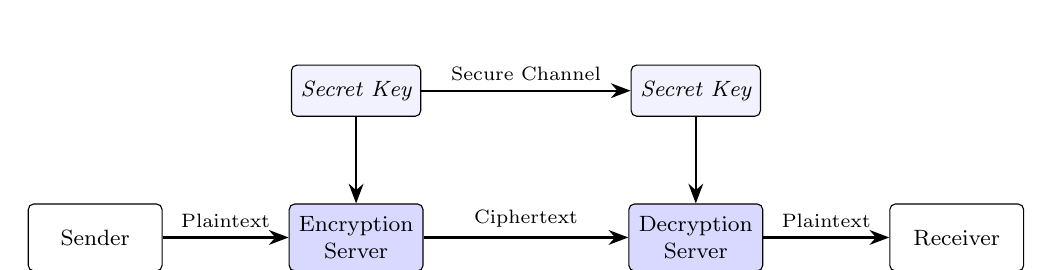
\begin{tikzpicture}[
    node distance=1.2cm and 1.6cm,
    box/.style={draw, rounded corners=2pt, minimum width=1.7cm, minimum height=0.85cm, align=center, font=\footnotesize},
    keyb/.style={draw, rounded corners=2pt, minimum width=1.5cm, minimum height=0.65cm, align=center, font=\footnotesize\itshape, fill=blue!5},
    ar/.style={-{Stealth[length=2.5mm]}, thick},
    font=\footnotesize
]
\node[box] (sender) {Sender};
\node[box, right=of sender, fill=blue!15] (enc) {Encryption\\Server};
\node[box, right=2.6cm of enc, fill=blue!15] (dec) {Decryption\\Server};
\node[box, right=of dec] (recv) {Receiver};
\node[keyb, above=1.1cm of enc] (k1) {Secret Key};
\node[keyb, above=1.1cm of dec] (k2) {Secret Key};
\draw[ar] (sender) -- node[above]{\scriptsize Plaintext} (enc);
\draw[ar, line width=1pt] (enc) -- node[above]{\scriptsize Ciphertext} (dec);
\draw[ar] (dec) -- node[above]{\scriptsize Plaintext} (recv);
\draw[ar] (k1) -- node[above, font=\scriptsize]{Secure Channel} (k2);
\draw[ar] (k1) -- (enc);
\draw[ar] (k2) -- (dec);
\end{tikzpicture}%
}
\vspace{.5em}
\caption{AES-256 encryption and decryption process using a symmetric secret key}
\label{fig:aes}
\end{figure}

\subsection{Compression algorithm implementation}
Compression uses a rule-based selection (\textit{rule-based decision tree}) rather than \textit{machine learning}, chosen for low \textit{overhead}, lightweight implementation, and fast, predictable decisions suited to low-latency backup. The algorithm is selected by file type and size (Table~\ref{tab:rule_selection}): small-to-medium text (CSV/LOG/TXT $\leq 100$~MB) to Snappy/LZ4 for speed; large text to Zstandard for ratio; already-compressed JPG to lightweight algorithms; XLSX to LZ4/Zstandard by size. A priority order with \textit{fallback} (Gzip as final safety net) guarantees every file is backed up. Five open-source algorithms are implemented in Python and applied identically to each file, measuring compression ratio and processing time \cite{36}, \cite{37}, \cite{38}, \cite{39}, \cite{22}.

\begin{table}[H]
\centering
\fontsize{8pt}{10pt}\selectfont
\caption{Compression algorithm selection rules by file type and size (priority order with \textit{fallback})}
\label{tab:rule_selection}
\begin{tabular}{l l l}
\hline
\textbf{File type} & \textbf{Size condition} & \textbf{Algorithm priority order} \\
\hline
CSV / LOG / TXT & $\leq 100$ MB & Snappy $\rightarrow$ LZ4 $\rightarrow$ Zstandard \\
CSV / LOG / TXT & $> 100$ MB & Zstandard $\rightarrow$ Gzip \\
JPG & all sizes & Snappy $\rightarrow$ LZ4 $\rightarrow$ Gzip \\
XLSX & $\leq 250$ MB & LZ4 $\rightarrow$ Zstandard \\
XLSX & $> 250$ MB & Zstandard $\rightarrow$ Gzip \\
Others & all sizes & Gzip (\textit{fallback}) \\
\hline
\end{tabular}
\end{table}

\subsection{Backup and recovery procedure}
Backup begins with SHA-256 baseline computation, then compression, then AES-256 encryption of the compressed output (\textit{compress-then-encrypt}); files are staged \textit{air-gapped} and mirrored to cloud. Under normal conditions (no anomaly), the system stops after backup, avoiding unnecessary recovery \textit{overhead}. Recovery is triggered only on anomalies (\textit{hash} mismatch, metadata inconsistency, unauthorized encryption): data are retrieved from \textit{air-gapped} storage, decrypted then decompressed, and validated against the baseline \textit{hash}. Figure~\ref{fig:backup_flow} shows the flowchart.

\begin{figure}[H]
\centering
\resizebox{0.86\textwidth}{!}{%
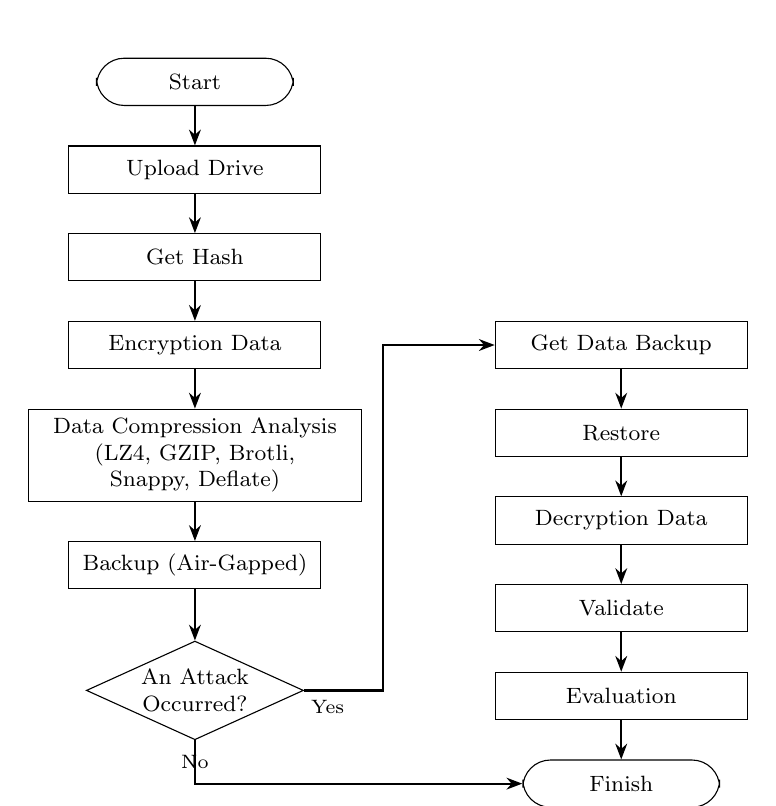
\begin{tikzpicture}[
    node distance=0.5cm,
    every node/.style={font=\footnotesize},
    term/.style={draw, rounded corners=10pt, minimum width=2.5cm, minimum height=0.6cm, align=center},
    proc/.style={draw, minimum width=3.2cm, minimum height=0.6cm, align=center},
    dec/.style={draw, diamond, aspect=2.2, inner sep=1pt, align=center},
    ar/.style={-{Stealth[length=2mm]}, thick}
]
\node[term] (start) {Start};
\node[proc, below=of start] (upload) {Upload Drive};
\node[proc, below=of upload] (hash) {Get Hash};
\node[proc, below=of hash] (enc) {Encryption Data};
\node[proc, below=of enc, text width=4.0cm] (comp) {Data Compression Analysis\\(LZ4, GZIP, Brotli, Snappy, Deflate)};
\node[proc, below=of comp] (backup) {Backup (Air-Gapped)};
\node[dec, below=0.65cm of backup] (att) {An Attack\\Occurred?};
\node[proc, right=2.2cm of enc] (getbk) {Get Data Backup};
\node[proc, below=of getbk] (restore) {Restore};
\node[proc, below=of restore] (decr) {Decryption Data};
\node[proc, below=of decr] (valid) {Validate};
\node[proc, below=of valid] (eval) {Evaluation};
\node[term, below=of eval] (finish) {Finish};
\draw[ar] (start) -- (upload);
\draw[ar] (upload) -- (hash);
\draw[ar] (hash) -- (enc);
\draw[ar] (enc) -- (comp);
\draw[ar] (comp) -- (backup);
\draw[ar] (backup) -- (att);
\draw[ar] (att.east) -- node[below, font=\scriptsize, pos=0.3]{Yes} ++(1.0cm,0) |- (getbk.west);
\draw[ar] (getbk) -- (restore);
\draw[ar] (restore) -- (decr);
\draw[ar] (decr) -- (valid);
\draw[ar] (valid) -- (eval);
\draw[ar] (eval) -- (finish);
\draw[ar] (att.south) |- node[below, font=\scriptsize, pos=0.05]{No} (finish.west);
\end{tikzpicture}%
}
\vspace{.5em}
\caption{Backup and recovery system flowchart}
\label{fig:backup_flow}
\end{figure}

\subsection{Ransomware attack simulation and detection}
Resilience was evaluated by simulating ransomware \textbf{without executing real \textit{malware}}, based on real vulnerability patterns: CVE-2017-0144 (\textit{encrypt-and-hold}), CVE-2021-36934 (overwrite/corruption), and CVE-2018-8453 (metadata/\textit{header} corruption). Files were modified in a controlled manner to mimic ransomware damage. Detection combines SHA-256 \textit{hash} verification, metadata analysis (size, modification time, type, extension), and \textit{air-gapped} backup validation. Each file's baseline \textit{hash} is re-verified during inspection; discrepancies between primary and \textit{air-gapped} copies classify a file as normal, legitimately modified, or a ransomware indication, enabling early detection and secure recovery.

\subsection{Performance evaluation metrics}
Storage efficiency uses Compression Ratio $CR=S_{after}/S_{before}$, Compression Factor $CF=S_{before}/S_{after}$, and Storage Saving $SS=(S_{before}-S_{after})/S_{before}\times100\%$. A combined efficiency score via a Multi-Criteria Decision Making Weighted Sum Model is $E=\alpha(1-R)+\beta(1/T)$ with $\alpha=\beta=0.5$ (balancing storage efficiency $1-R$ and time efficiency $1/T$), normalized as $E(\%)=E/E_{max}\times100$; Table~\ref{tab:efficiency_criteria} lists the interpretation. Recovery is measured by $RTO=T_{recovery}-T_{incident}$. Detection reliability uses $FPR=FP/(FP+TN)\times100\%$ and $FNR=FN/(FN+TP)\times100\%$, where lower values indicate higher reliability.

\begin{table}[H]
\centering
\fontsize{8pt}{10pt}\selectfont
\caption{Criteria for interpreting system efficiency score}
\label{tab:efficiency_criteria}
\begin{tabularx}{\textwidth}{@{}c c X@{}}
\hline
\textbf{Score (\%)} & \textbf{Status} & \textbf{Description} \\
\hline
$\geq 90$ & Excellent & Very high performance in both storage efficiency and speed \\
80--89 & Good & Strong performance for high-performance systems \\
70--79 & Fair & One aspect dominant, the other weaker \\
$< 70$ & Poor & Overall efficiency is low \\
\hline
\end{tabularx}
\end{table}

\section{Results and Discussion}
\label{sec:results}
The proposed system delivered reliable protection, compression, and recovery: all files kept identical SHA-256 \textit{hash} values (zero alteration), Zstandard/Brotli gave the highest compression while Snappy/LZ4 were fastest, and the \textit{air-gapped} mechanism enabled 100\% recovery with zero errors under simulation.

\subsection{Experimental environment}
The system was evaluated in two environments: a local \textbf{Windows} development environment and a \textbf{cloud} replication on AWS EC2 (Windows Server and Linux). Cloud replication is directly relevant since the system targets cloud backup. Table~\ref{tab:experimental_setup} summarizes both.

\begin{table}[H]
\centering
\fontsize{8pt}{10pt}\selectfont
\caption{Experimental setup across two test environments}
\label{tab:experimental_setup}
\begin{tabularx}{\textwidth}{@{}l X X@{}}
\hline
\textbf{Component} & \textbf{Local (Windows)} & \textbf{Cloud (AWS EC2)} \\
\hline
Operating System & Windows 11 (64-bit) & Windows Server 2022 \& Ubuntu 22.04 \\
CPU & Intel Core i7-11800H (8-core) & t3.xlarge (4 vCPU) / t3.large (2 vCPU) \\
RAM & 16 GB & 16 GB (Windows) / 8 GB (Linux) \\
Language & Python 3.10 & Python 3.11 / 3.10 \\
Compression & \multicolumn{2}{l}{Gzip, Zstandard, Brotli, LZ4, Snappy} \\
Cryptography & \multicolumn{2}{l}{PyCryptodome (AES-256), hashlib (SHA-256)} \\
\textit{Air-gapped} Media & External SSD / VHDX & Separate EBS volume (D: / \texttt{/mnt/airgap}) \\
Cloud Storage & Google Drive API & Amazon S3 \\
\hline
\end{tabularx}
\end{table}

The Windows machine is the \textbf{initial development environment}, while AWS EC2 is the \textbf{primary measurement/validation environment}: all reported quantitative figures (ratio, \textit{throughput}, RTO, repeated-trial statistics) come from controlled EC2 measurements. Testing on two platforms verifies cross-platform consistency and mitigates the single-platform generalizability limitation.

\subsection{Normal conditions (no attack)}
The main workflow was verified end-to-end. The system establishes a secure cloud connection via token/role-based authentication (OAuth~2.0 for Google Drive; IAM \textit{role} for S3), generating a unique session ID per backup (Figure~\ref{fig:drive_conn}). It then uploads and validates files with SHA-256 \textit{hashing} and metadata before compression/encryption (Figure~\ref{fig:upload}), ensuring only valid files are processed and reducing redundancy.

\begin{figure}[H]
\centering
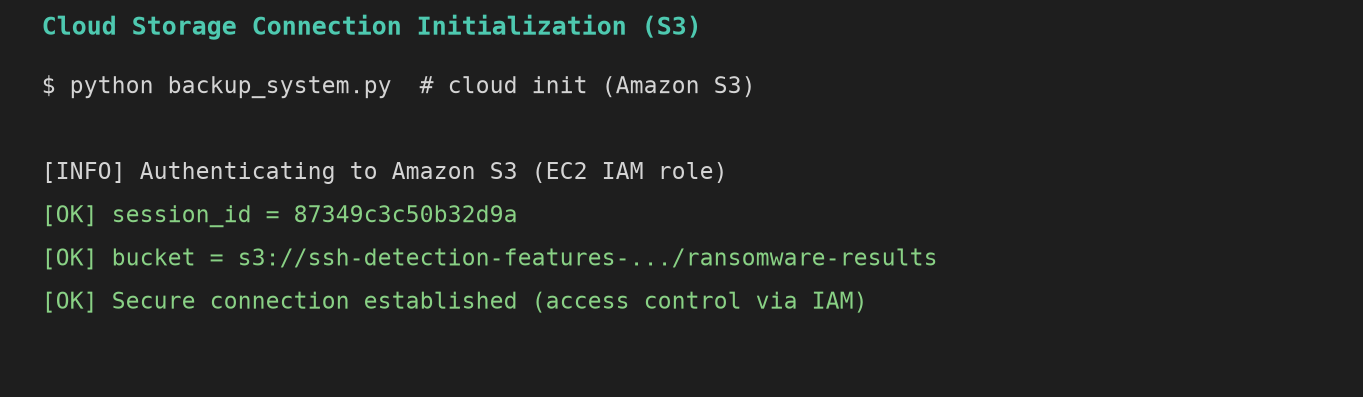
\includegraphics[width=0.62\textwidth]{figures/figure4_cloud_conn_en.png}
\vspace{.4em}
\caption{Drive connection results (session ID)}
\label{fig:drive_conn}
\end{figure}

\begin{figure}[H]
\centering
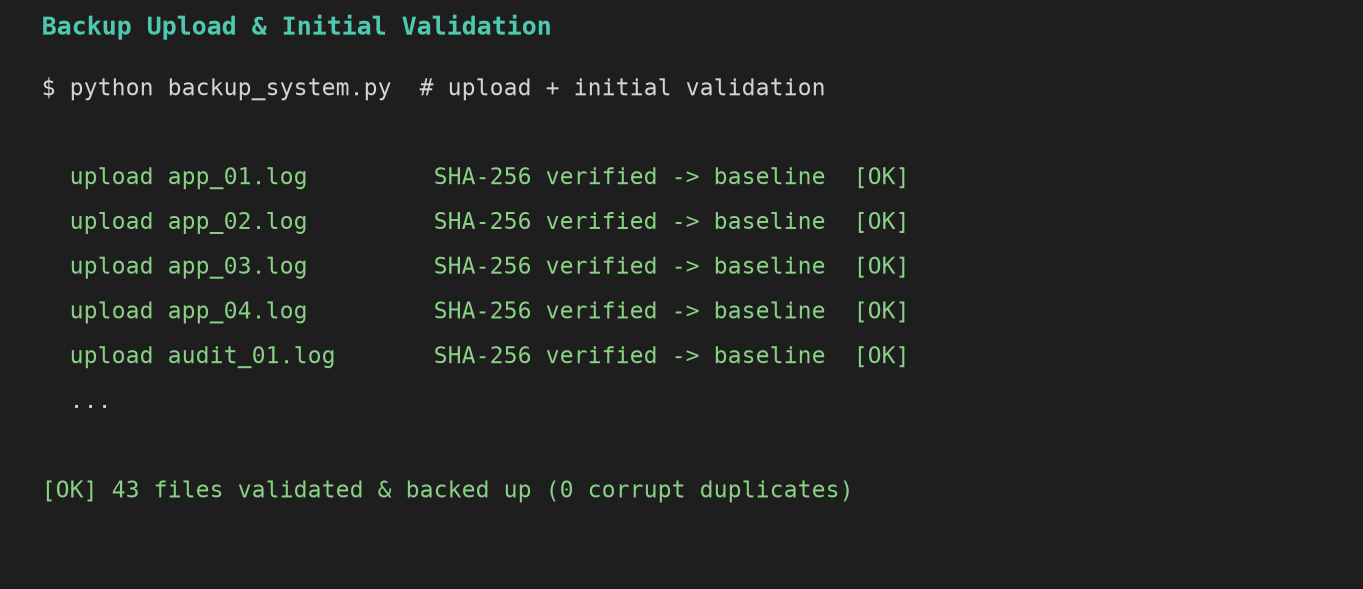
\includegraphics[width=0.62\textwidth]{figures/figure5_upload_en.png}
\vspace{.4em}
\caption{Backup upload and initial validation results}
\label{fig:upload}
\end{figure}

Integrity validation computes a unique SHA-256 \textit{hash} per file as a digital fingerprint (Figure~\ref{fig:sha_json}), stored together with metadata (size, timestamp, MIME type, extension, structure) as a JSON baseline (Figure~\ref{fig:metadata}). Algorithm~1 summarizes the validation: any \textit{hash}/metadata deviation from the baseline flags an anomaly.

\begin{figure}[H]
\centering
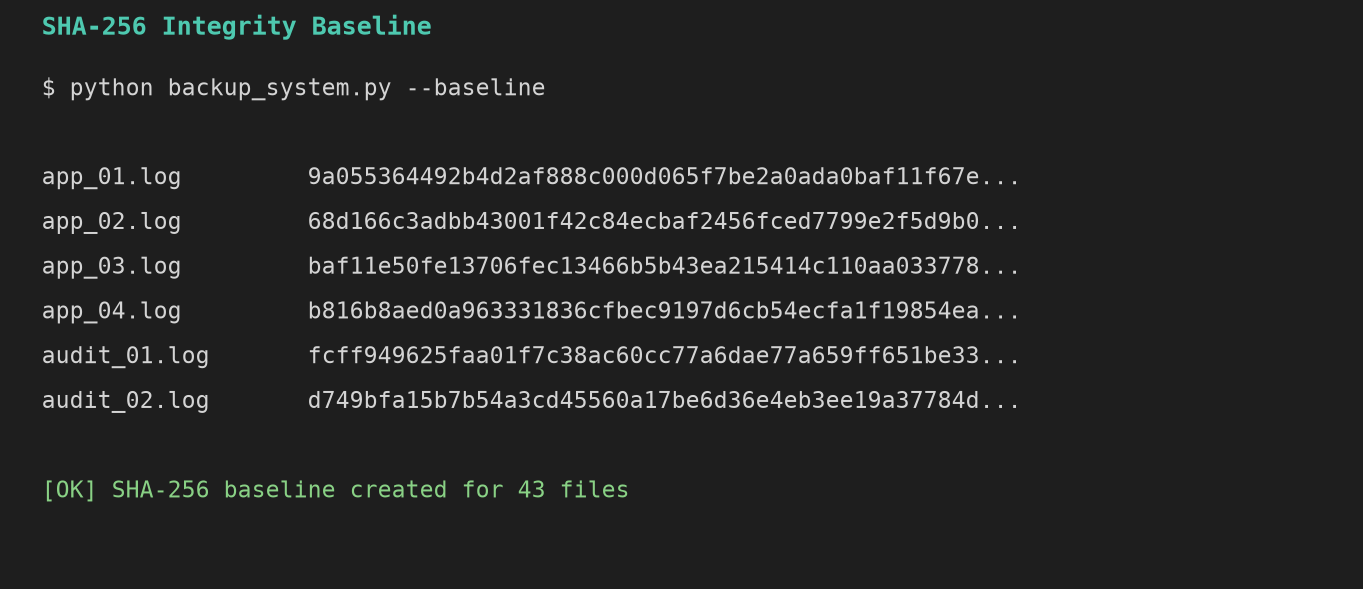
\includegraphics[width=0.62\textwidth]{figures/figure6_sha256_en.png}
\vspace{.4em}
\caption{SHA-256 results for the JSON file}
\label{fig:sha_json}
\end{figure}

\begin{figure}[H]
\centering
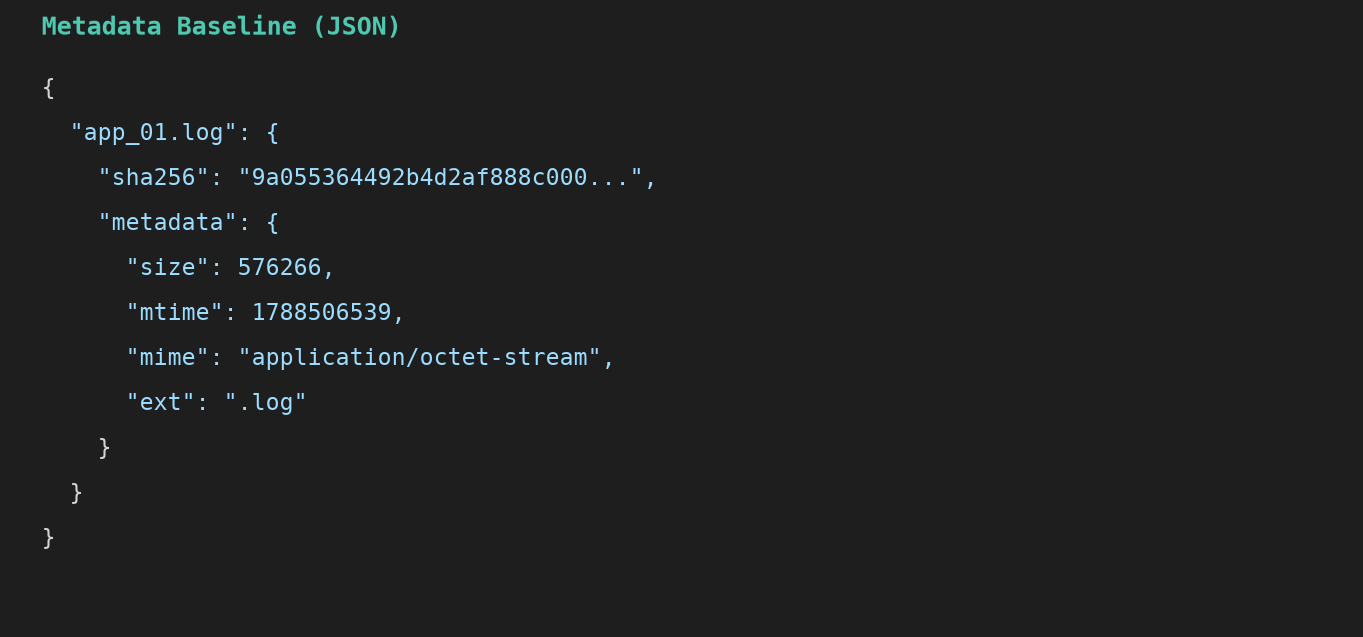
\includegraphics[width=0.55\textwidth]{figures/figure7_metadata.png}
\vspace{.4em}
\caption{Metadata results in JSON format}
\label{fig:metadata}
\end{figure}

\begin{table}[H]
\centering
\fontsize{8pt}{10pt}\selectfont
\begin{tabularx}{\textwidth}{@{}X@{}}
\hline
\textbf{Algorithm 1. Hash and metadata validation process} \\
\hline
FOR each file IN dataset: \quad hash = SHA256(file); \quad metadata = extract\_metadata(file) \\
\quad IF hash or metadata differ from baseline: mark\_as\_anomaly(file) \quad ELSE: mark\_as\_safe(file) \\
\hline
\end{tabularx}
\end{table}

This combination detects content-level and structural changes (altered timestamps, suspicious extensions, corrupted headers). Figure~\ref{fig:validation} confirms all files were verified with \texttt{detected\_ransom\_files: []}, i.e., safe before compression/encryption.

\begin{figure}[H]
\centering
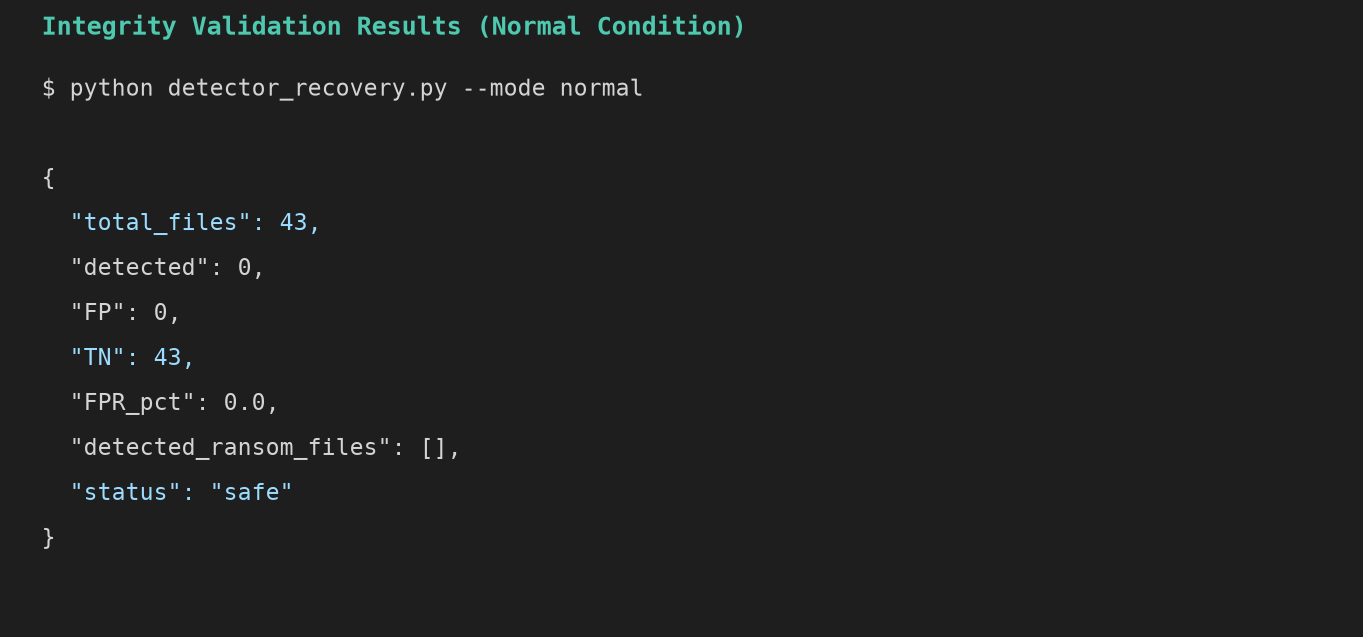
\includegraphics[width=0.55\textwidth]{figures/figure8_validation_en.png}
\vspace{.4em}
\caption{Validation results of SHA-256 hash and file metadata}
\label{fig:validation}
\end{figure}

The system then applies AES-256 to verified files, producing \texttt{.enc} outputs (Figure~\ref{fig:aes_log}); Algorithm~2 summarizes the workflow. Encryption runs only after successful \textit{hash}/metadata validation, so legitimate backup encryption (authorized keys, verified files) is cleanly distinguished from ransomware behavior.

\begin{figure}[H]
\centering
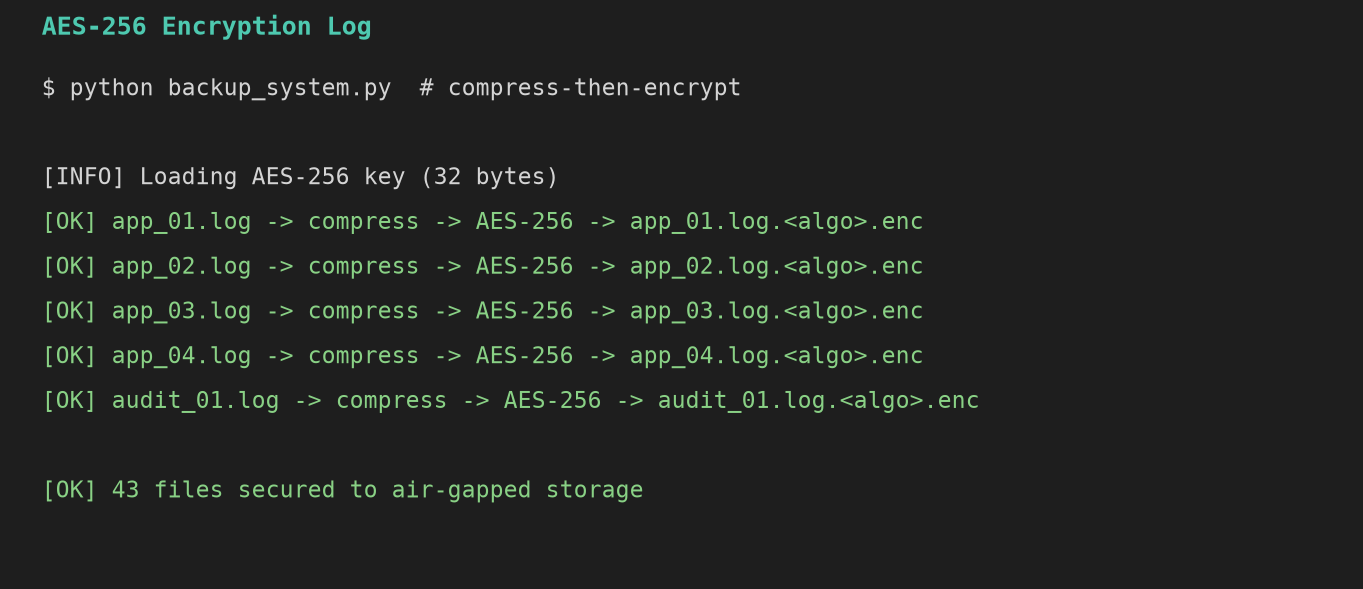
\includegraphics[width=0.62\textwidth]{figures/figure9_aeslog_en.png}
\vspace{.4em}
\caption{Log of the file encryption implementation using the AES-256 algorithm}
\label{fig:aes_log}
\end{figure}

\begin{table}[H]
\centering
\fontsize{8pt}{10pt}\selectfont
\begin{tabularx}{\textwidth}{@{}X@{}}
\hline
\textbf{Algorithm 2. AES-256 encryption process} \\
\hline
LOAD encryption\_key \\
FOR each validated\_file IN dataset: \quad encrypted\_file = AES256\_Encrypt(validated\_file, encryption\_key) \\
\quad save(encrypted\_file, ".enc"); \quad log\_encryption\_status(encrypted\_file) \\
\hline
\end{tabularx}
\end{table}

\subsection{Compression performance by algorithm}
Table~\ref{tab:compression_results} reports the average storage saving (SS) at the \textit{plaintext} stage for each file type and algorithm.

\begin{table}[H]
\centering
\fontsize{8pt}{10pt}\selectfont
\caption{Average storage saving (\%) by file type and algorithm (43 files)}
\label{tab:compression_results}
\begin{tabular}{l c c c c c}
\hline
\textbf{File Type} & \textbf{Gzip} & \textbf{Zstandard} & \textbf{Brotli} & \textbf{LZ4} & \textbf{Snappy} \\
\hline
Log/TXT & 88.5 & 87.6 & \textbf{89.5} & 77.4 & 80.2 \\
CSV     & 79.9 & 78.7 & \textbf{81.1} & 66.6 & 66.4 \\
XLSX    & 1.1  & 0.0  & 0.0  & 0.0  & 0.0  \\
JPG     & 0.1  & 0.0  & 0.0  & 0.0  & 0.0  \\
\hline
\end{tabular}
\end{table}

Low-entropy text yields the highest savings (Log/TXT up to \textbf{89.5\%}, CSV up to \textbf{81.1\%} with Brotli; Gzip/Zstandard follow closely above 78\%). Fast algorithms (LZ4/Snappy) give slightly lower savings (66--80\%) at far shorter times---ideal for real-time scenarios. JPG and XLSX (already compressed) approach \textbf{0\%}, confirming the \textit{lossless} limit on high-entropy data and validating the rule-based adaptive selection (Figure~\ref{fig:overall_analysis}).

\begin{figure}[H]
\centering
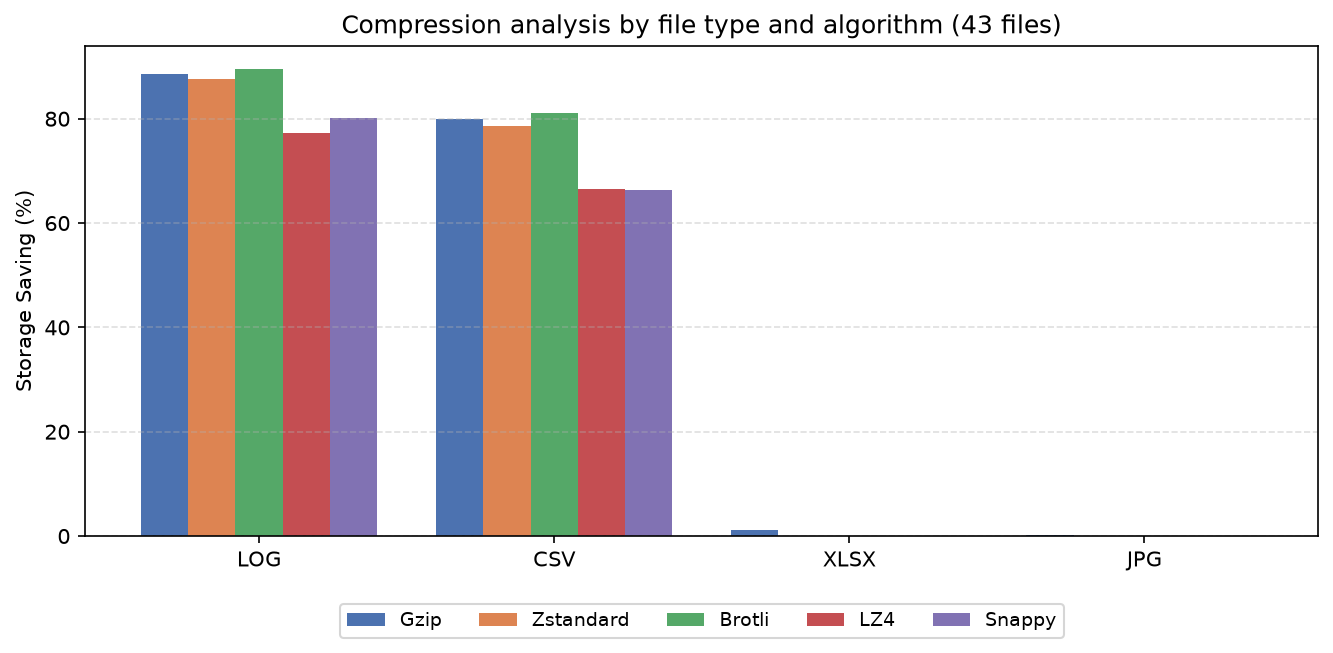
\includegraphics[width=0.62\textwidth]{figures/figure10_compression_en.png}
\vspace{.4em}
\caption{Overall analysis results of the algorithms}
\label{fig:overall_analysis}
\end{figure}

\subsection{Statistical analysis of compression performance}
Compression was repeated five times on the full \textit{dataset} (43 files, $\approx531$~MB) on AWS EC2 (Ubuntu 22.04). Table~\ref{tab:comp_stats} reports mean$\pm$std of time, \textit{throughput}, and CPU/RAM (via \texttt{psutil}).

\begin{table}[H]
\centering
\fontsize{8pt}{10pt}\selectfont
\caption{Statistical analysis of compression performance (5 trials, 43 files $\approx$531 MB)}
\label{tab:comp_stats}
\begin{tabular}{l c c c c c}
\hline
\textbf{Algorithm} & \textbf{Mean time (s)} & \textbf{Std (s)} & \textbf{Throughput (MB/s)} & \textbf{CPU (\%)} & \textbf{RAM (MB)} \\
\hline
Gzip      & 17.427 & 0.062 & 30.5  & 100.0 & 6.3 \\
Brotli    & 10.468 & 0.237 & 50.7  & 100.0 & 5.1 \\
Zstandard & 1.721  & 0.016 & 308.7 & 99.9  & 3.4 \\
LZ4       & 0.896  & 0.011 & 592.7 & 100.0 & $<$1 \\
Snappy    & 0.831  & 0.003 & 639.0 & 99.3  & 0.9 \\
\hline
\end{tabular}
\end{table}

The very small std (e.g., Snappy 0.003~s, Zstandard 0.016~s) shows stable, consistent performance. \textit{Throughput} spans a wide range (Snappy/LZ4 $>590$~MB/s, $\approx20\times$ Gzip's 30.5~MB/s), while Zstandard balances speed (308.7~MB/s) with a high ratio. Near-100\% CPU confirms the process is \textit{CPU-bound}; small RAM ($<7$~MB) keeps it lightweight for constrained environments---an objective basis for adaptive selection.

\subsection{Comparison against baselines}
The adaptive strategy was compared to (i) no compression, (ii) static Gzip, and (iii) static Zstandard on the full \textit{dataset} (Table~\ref{tab:baseline_comparison}).

\begin{table}[H]
\centering
\fontsize{8pt}{10pt}\selectfont
\caption{Comparison of the adaptive strategy against baselines (43 files, $\approx$531 MB)}
\label{tab:baseline_comparison}
\begin{tabular}{l c c c c}
\hline
\textbf{Strategy} & \textbf{Final Size (MB)} & \textbf{Saving (\%)} & \textbf{Time (s)} & \textbf{Throughput (MB/s)} \\
\hline
No compression        & 531.2 & 0.00  & --    & -- \\
Static-Gzip           & 265.1 & 50.09 & 18.84 & 28.2 \\
Static-Zstandard      & 271.1 & 48.96 & 1.94  & 273.8 \\
\textbf{Adaptive (proposed)} & 301.3 & 43.28 & \textbf{0.87} & \textbf{611.8} \\
\hline
\end{tabular}
\end{table}

Static Gzip achieves the highest saving (50.1\%) but is slow (18.84~s; 28.2~MB/s). The adaptive strategy prioritizes speed---finishing in 0.87~s, \textbf{$\approx21\times$ faster than static Gzip} and $2.2\times$ faster than static Zstandard---while still saving 43.3\%. Trading 6.8 percentage points of saving for a dramatic \textit{throughput} gain (611.8 vs 28.2~MB/s) is advantageous for low-RTO, resource-constrained backup. The adaptive mechanism's key benefit is thus the \textbf{optimal balance} between storage efficiency and speed.

\subsection{Entropy analysis}
Shannon entropy $H(X)$ (bits/\textit{byte}, 0--8) per file type is related to saving in Table~\ref{tab:entropy_type} and to attack detection in Table~\ref{tab:entropy_attack}.

\begin{table}[H]
\centering
\fontsize{8pt}{10pt}\selectfont
\caption{Shannon entropy per file type and its relation to storage saving}
\label{tab:entropy_type}
\begin{tabular}{l c c}
\hline
\textbf{File Type} & \textbf{Entropy (bits/byte)} & \textbf{Saving (\%)} \\
\hline
CSV  & 4.573 & 66.4 \\
LOG  & 5.232 & 80.0 \\
XLSX & 7.962 & $\approx$0 \\
JPG  & 7.940 & $\approx$0 \\
\hline
\end{tabular}
\end{table}

\begin{table}[H]
\centering
\fontsize{8pt}{10pt}\selectfont
\caption{Shannon entropy change before and after ransomware encryption attack}
\label{tab:entropy_attack}
\begin{tabular}{l c c c}
\hline
\textbf{File Type} & \textbf{Before} & \textbf{After} & \textbf{$\Delta H$} \\
\hline
CSV  & 4.547 & 8.000 & $+3.453$ \\
LOG  & 5.223 & 8.000 & $+2.777$ \\
JPG  & 7.940 & 8.000 & $+0.060$ \\
XLSX & 7.963 & 8.000 & $+0.036$ \\
\hline
\end{tabular}
\end{table}

Text files (CSV, LOG) have low entropy (4.6--5.2) and compress by 66--80\%, while JPG/XLSX near the 8.0 limit barely compress---a strong inverse correlation justifying file-type-based selection. After an \textit{encrypt-and-hold} attack, low-entropy files spike to 8.0 ($\Delta H$ up to $+3.45$), a clear sign of unauthorized encryption; already-high-entropy files change little, exposing the weakness of entropy-only detection (e.g., FPE) and reinforcing our reliance on \textit{hash}/metadata integrity, which detects \textit{any} change regardless of entropy.

\subsection{Recovery time scalability}
The backup--recovery cycle was measured from 50~MB to 1~GB (Table~\ref{tab:scalability}).

\begin{table}[H]
\centering
\fontsize{8pt}{10pt}\selectfont
\caption{Scalability of backup and recovery time (RTO) with dataset size}
\label{tab:scalability}
\begin{tabular}{c c c c}
\hline
\textbf{Dataset (MB)} & \textbf{Backup (s)} & \textbf{Recovery RTO (s)} & \textbf{Recovered} \\
\hline
51.2   & 0.187 & 0.344 & 8/8 \\
101.1  & 0.339 & 0.699 & 8/8 \\
250.9  & 0.872 & 1.797 & 8/8 \\
500.5  & 1.843 & 4.020 & 8/8 \\
1001.0 & 5.927 & 7.731 & 8/8 \\
\hline
\end{tabular}
\end{table}

RTO grows \textbf{approximately linearly} ($\approx0.0073$~s/MB, std only 0.0005), confirming the deterministic workflow (SHA-256, AES-256 decryption, decompression). Even a 1~GB \textit{dataset} recovers fully in $\approx7.7$~s with integrity preserved, enabling reliable RTO projection for enterprise scale.

\subsection{Air-gapped backup storage implementation and structure}
As an added protection layer, the system implements a \textbf{logical (online) air-gap} on a separate medium (external SSD/VHDX) that is not permanently accessible: it is \textit{mounted} only during a backup or restore session, minimizing unauthorized access and network-borne \textit{malware} propagation. The medium stays within the system environment but is reachable only under system-defined conditions (access control, active sessions, limited \textit{mounting}) with no active network connection during storage. This is not as strong as a fully offline physical \textit{air-gap}---advanced \textit{memory-resident} \textit{malware} could attempt access while the medium is mounted---but the residual risk is mitigated by short \textit{mount} durations, automatic disconnection after backup, SHA-256/metadata verification, isolated repositories, and restricted sessions, offering a practical, cost-effective option for small and medium organizations. Figure~\ref{fig:airgap_storage} shows the structure: backups organized by compression algorithm, plus a JSON \textit{hash-storage} file holding SHA-256 values of original and backup files for integrity validation on isolated media.

\begin{figure}[H]
\centering
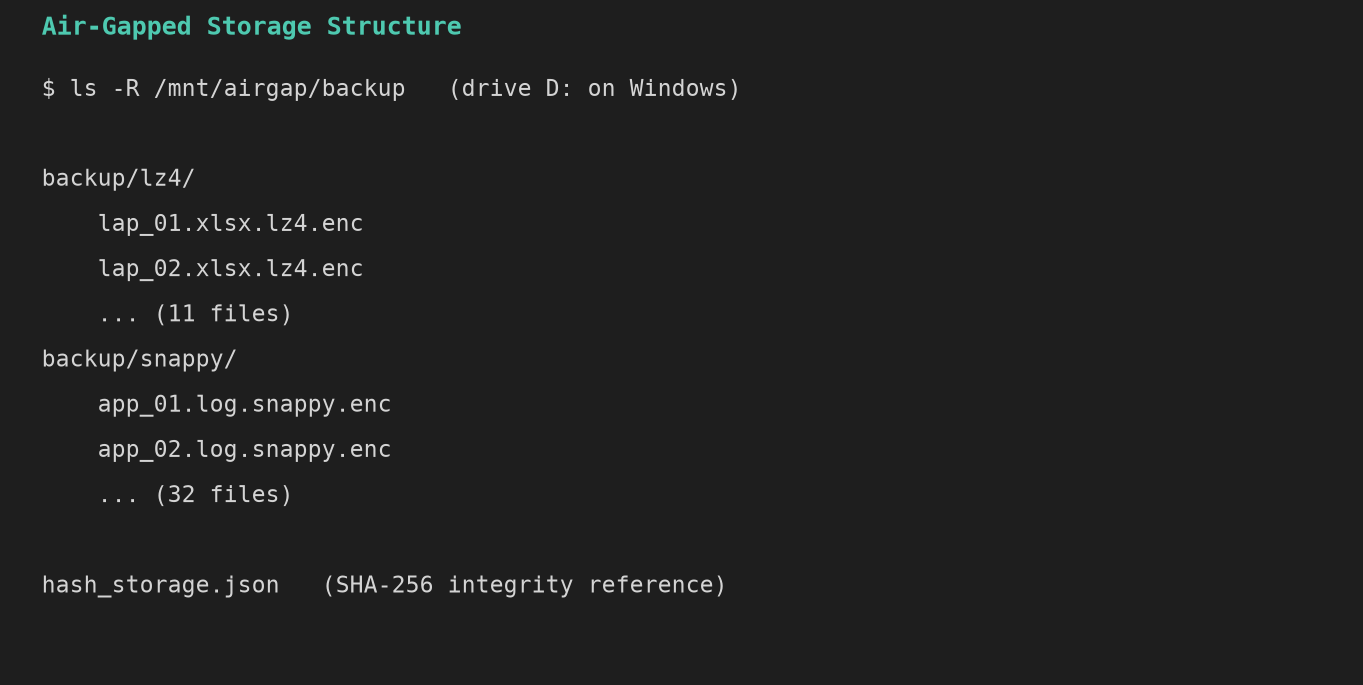
\includegraphics[width=0.6\textwidth]{figures/figure11_airgap_struct_en.png}
\vspace{.4em}
\caption{Air-gapped online storage}
\label{fig:airgap_storage}
\end{figure}

\subsection{Transfer and logging to air-gapped storage}
Transfers to \textit{air-gapped} storage are controlled and logged automatically, recording the reset/\textit{mounting} stages and the subsequent short data transfer. Figure~\ref{fig:transfer} shows the destination, processing time, and success status; this logging enables detailed audit and trace of backup activity, evidencing that transfers to \textit{air-gapped} media are performed separately rather than continuously.

\begin{figure}[H]
\centering
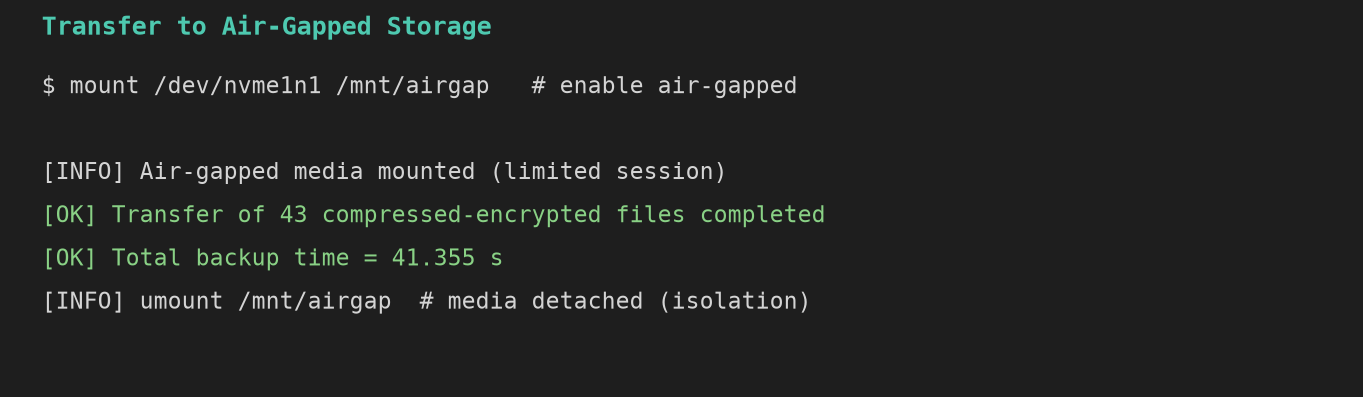
\includegraphics[width=0.6\textwidth]{figures/figure12_transfer_en.png}
\vspace{.4em}
\caption{Transfer to air-gapped storage}
\label{fig:transfer}
\end{figure}

\subsection{System monitoring and integrity validation}
Monitoring uses an interactive \textit{dashboard} (Figure~\ref{fig:dashboard}) summarizing file status, compression ratio, compression time, validation results, and restore status per algorithm in real time. During the simulation the system detected no anomalies in structure or metadata (size, format/extension, last-modified timestamp), and matching SHA-256 \textit{hashes} confirmed no content change or corruption during backup.

\begin{figure}[H]
\centering
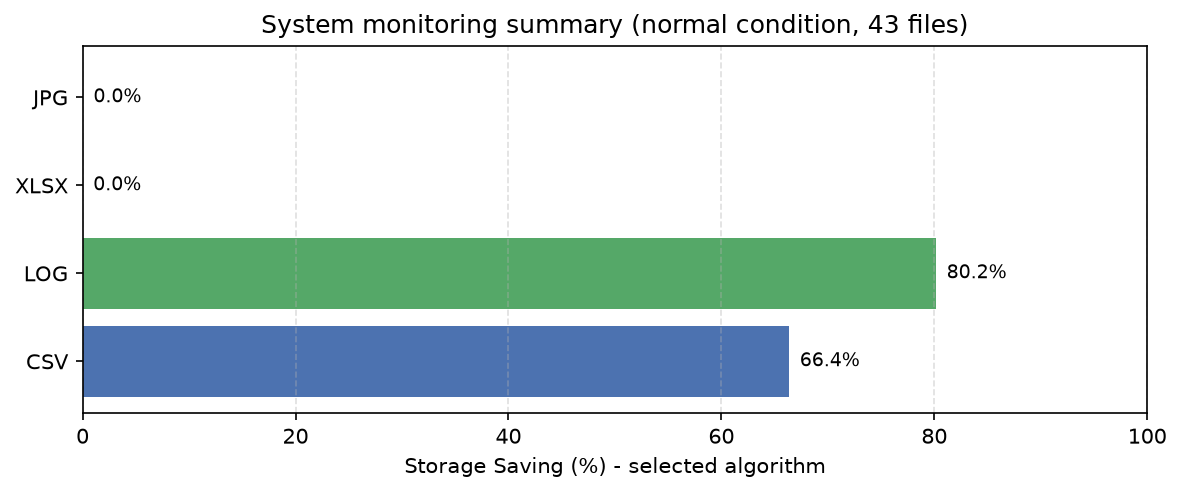
\includegraphics[width=0.6\textwidth]{figures/figure13_dashboard_en.png}
\vspace{.4em}
\caption{System monitoring dashboard under normal conditions (no attack)}
\label{fig:dashboard}
\end{figure}

\subsection{Simulation under disrupted conditions (ransomware attack)}
Under disrupted conditions, main-system files were corrupted by simulated attacks while backups remained secure in isolated \textit{air-gapped} storage; on detecting \textit{hash}/metadata anomalies the system automatically referred to backup copies for recovery.

\subsubsection{File damage simulation}
Three damage types were tested on small-to-medium files (Table~\ref{tab:damage_simulation}). The backup mechanism preserved integrity or enabled recovery from \textit{air-gapped} backups even when original content was partially or fully damaged.

\begin{table}[H]
\centering
\fontsize{8pt}{10pt}\selectfont
\caption{Results of file damage simulation due to ransomware attacks}
\label{tab:damage_simulation}
\begin{tabularx}{\textwidth}{@{}>{\raggedright\arraybackslash}p{2.2cm} >{\raggedright\arraybackslash}p{1.9cm} >{\raggedright\arraybackslash}X >{\raggedright\arraybackslash}X >{\raggedright\arraybackslash}X@{}}
\hline
\textbf{Attack Type} & \textbf{File Target} & \textbf{Simulation Method} & \textbf{Scenario Observation} & \textbf{Result} \\
\hline
Encrypt and Hold (CVE-2017-0144) & finance\_\-log\_\-500kb.log & Controlled modification of file content to simulate WannaCry encryption patterns & File changes to WNCRY format, timestamp modified to 11/12/2025 09:58 & Files become unreadable; hash differs from original \\
Metadata/Header Corruption (CVE-2018-8453) & finance\_\-log\_\-500kb.log & Controlled modification of file headers & Initial part corrupted with random characters; lower part still shows valid log entries & Initial part corrupted; lower part still readable \\
Overwrite-and-Corrupt (CVE-2021-36934) & finance\_\-log\_\-500kb.log & Controlled overwriting of partial content with random characters & Log structure disorganized; some INFO/ERROR/DEBUG remain; non-ASCII characters appear & Files unrecoverable; hash differs \\
Recovery Validation & finance\_\-log\_\-500kb.log & Restoration from air-gapped backup & --- & Original file successfully recovered \\
\hline
\end{tabularx}
\end{table}

Each attack has a distinct impact: \textit{encrypt-and-hold} fully modifies content (size and timestamp change, unreadable); metadata/\textit{header} corruption damages the initial structure (partially readable); \textit{overwrite-and-corrupt} inserts random/non-ASCII characters, making recovery from the primary copy impossible---hence the need for isolated backups.

\subsubsection{Hash and metadata change analysis}
All attacked files produced SHA-256 \textit{hashes} differing from their baselines across all three scenarios, confirming that \textit{hash}-based integrity checking accurately detects content change even for partial damage; several metadata attributes also changed. Table~\ref{tab:hash_before} gives the baseline and Table~\ref{tab:hash_after} the post-attack values.

\begin{table}[H]
\centering
\fontsize{8pt}{10pt}\selectfont
\caption{Hash and metadata of file before simulation (integrity baseline)}
\label{tab:hash_before}
\begin{tabularx}{\textwidth}{@{}X c c c@{}}
\hline
\textbf{File} & \textbf{SHA-256 Hash} & \textbf{File Size} & \textbf{Last Modified / MIME Type} \\
\hline
finance\_log\_500KB.log & cd5bda6156e87c84971e9a5e3500d521 & 500 KB & 2025-12-04 10:08:36 (UTC) / text/plain \\
\hline
\end{tabularx}
\end{table}

\begin{table}[H]
\centering
\fontsize{8pt}{10pt}\selectfont
\caption{Hash and metadata of file after simulation}
\label{tab:hash_after}
\begin{tabularx}{\textwidth}{@{}p{2.3cm} >{\raggedright\arraybackslash}X c >{\raggedright\arraybackslash}p{2.2cm} >{\raggedright\arraybackslash}X@{}}
\hline
\textbf{Attack Type} & \textbf{SHA-256 Hash (truncated)} & \textbf{File Size} & \textbf{Last Modified} & \textbf{Status / Description} \\
\hline
Encrypt and Hold (CVE-2017-0144) & \texttt{2eb4e7bd18f290\-b66150a0d0d49\-bd79c} & 667 KB & 2026-01-06 20:56:49 & Changed; suspicious extension (MIME text/plain) \\
Metadata/Header Corruption (CVE-2018-8453) & \texttt{102453959e6585\-3e9257b095b9\-fcc27d048906} & 501 KB & 2026-01-14 20:22:08 & Changed; SHA-256 mismatch, file may be encrypted \\
Overwrite-and-Corrupt (CVE-2021-36934) & \texttt{fc5f9e8b9c532f\-94acefedfdd7\-b11a91707634} & 501 KB & 2026-01-17 09:02:37 & Changed; SHA-256 mismatch, file may be encrypted \\
\hline
\end{tabularx}
\end{table}

\subsubsection{System response to corrupted files}
The system auto-detects corrupted files by comparing \textit{checksums} before and after recovery; on mismatch it marks the file as failed and activates \textit{air-gapped} recovery, restoring all files from the isolated repository. Status is reported in JSON and via \textit{dashboard} notifications---e.g., \texttt{restore\_mode}=\{mode: "airgap", reason: "ransomware\_detected", scope: "all"\}, \texttt{airgap}=true, total restore 43, restore OK 43, errors 0. The \textit{frontend} shows a clear warning that a FULL RESTORE from isolated backup is in progress and the count of recovered files (Figure~\ref{fig:ui_restore}), so corrupted files do not compromise overall integrity.

\begin{figure}[H]
\centering
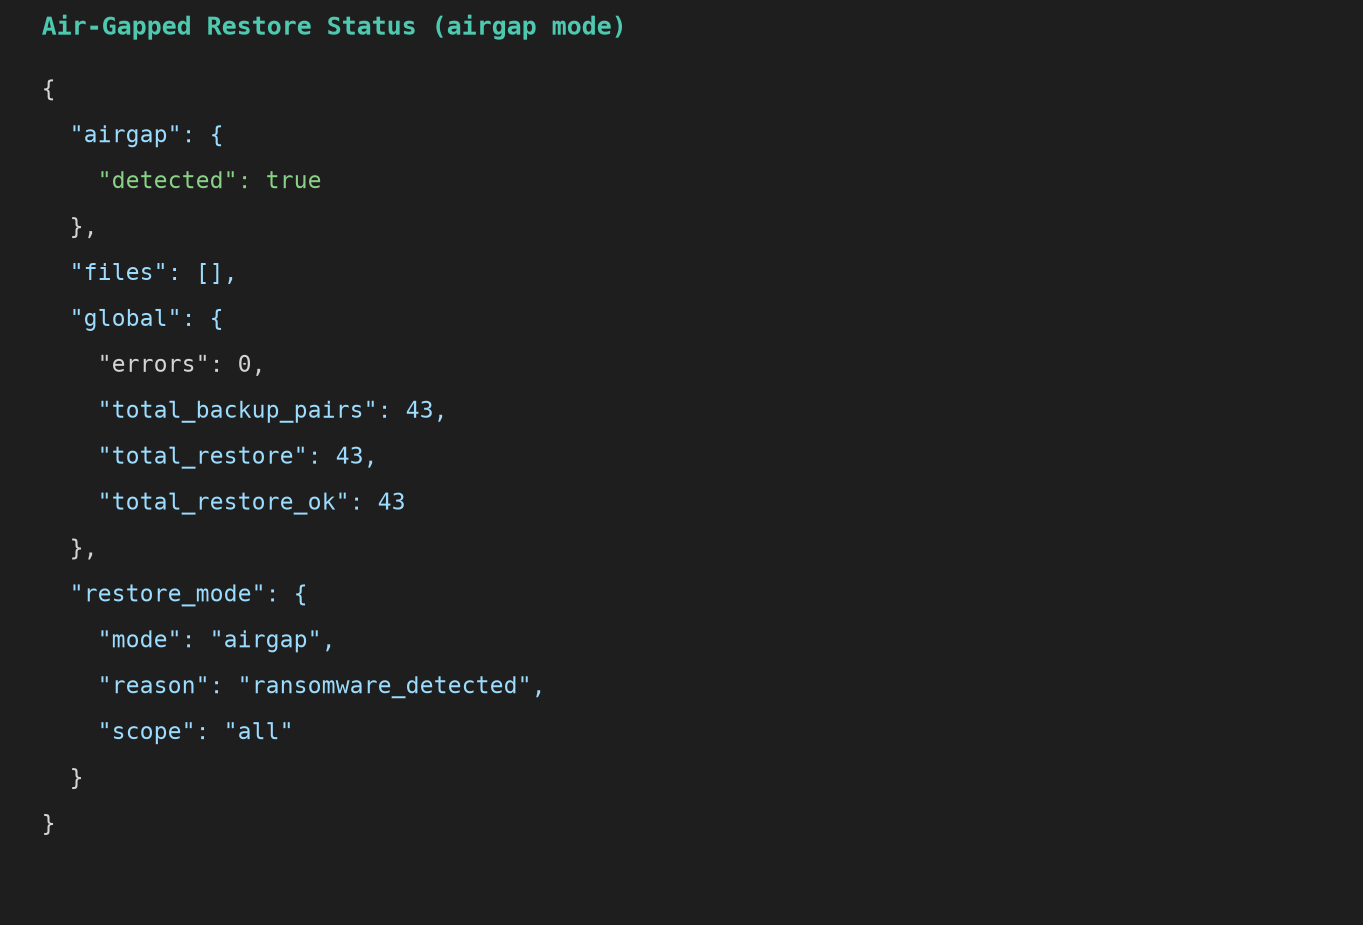
\includegraphics[width=0.6\textwidth]{figures/figure14_restore_json_en.png}
\vspace{.4em}
\caption{User interface showing restore status in air-gapped mode}
\label{fig:ui_restore}
\end{figure}

\subsection{Restore process from air-gapped backup}
After activating \textit{air-gapped} recovery, data are restored from physically and logically isolated media. Here the \textit{air-gap} is realized on a dedicated medium (Disk~G:) used exclusively as an isolated repository, not for normal operations and accessed only during recovery. Figure~\ref{fig:vhdx} shows the architecture: under normal conditions backup/restore use the directly connected primary repository, but on detecting corruption or ransomware indications the restore path switches to the isolated \textit{air-gapped} repository, separated from the main system and network.

\begin{figure}[H]
\centering
\resizebox{0.78\textwidth}{!}{%
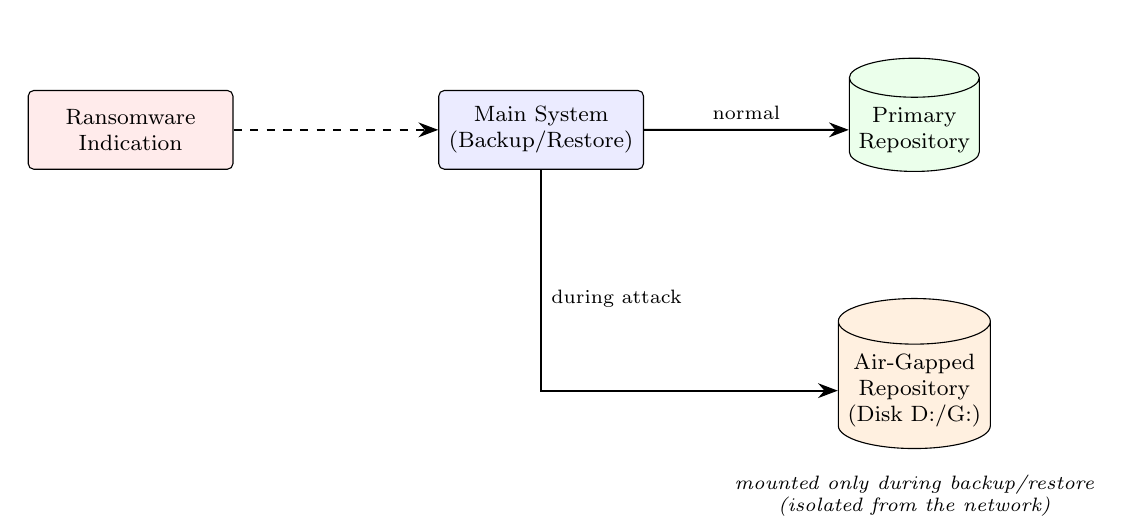
\begin{tikzpicture}[
    font=\footnotesize,
    box/.style={draw, rounded corners=2pt, minimum width=2.6cm, minimum height=1cm, align=center},
    store/.style={draw, cylinder, shape border rotate=90, aspect=0.3, minimum width=1.6cm, minimum height=1.4cm, align=center},
    ar/.style={-{Stealth[length=2.5mm]}, thick},
    ard/.style={-{Stealth[length=2.5mm]}, thick, dashed}
]
\node[box, fill=blue!8] (sys) {Main System\\(Backup/Restore)};
\node[store, right=2.6cm of sys, fill=green!8] (primary) {Primary\\Repository};
\node[store, below=1.6cm of primary, fill=orange!12] (airgap) {Air-Gapped\\Repository\\(Disk D:/G:)};
\node[box, left=2.6cm of sys, fill=red!8] (att) {Ransomware\\Indication};
\draw[ar] (sys) -- node[above]{\scriptsize normal} (primary);
\draw[ard] (att) -- (sys);
\draw[ar] (sys.south) |- node[below right, font=\scriptsize, pos=0.25]{\scriptsize during attack} (airgap.west);
\node[align=center, below=0.2cm of airgap, font=\scriptsize\itshape] {mounted only during backup/restore\\(isolated from the network)};
\end{tikzpicture}%
}
\vspace{.4em}
\caption{VHDX media-based air-gapped backup architecture with network separation}
\label{fig:vhdx}
\end{figure}

\subsection{Decompression, decryption, integrity validation, and recovery time}
Files recovered from the \textit{air-gapped} medium are compressed-and-encrypted, so the system first decrypts (AES-256) then decompresses, and validates by comparing SHA-256 \textit{checksums} before (sha\_in) and after (sha\_out) recovery; a file is valid when both match. Figure~\ref{fig:restore_terminal} shows all files recovered with status [OK]---43 files restored without errors.

\begin{figure}[H]
\centering
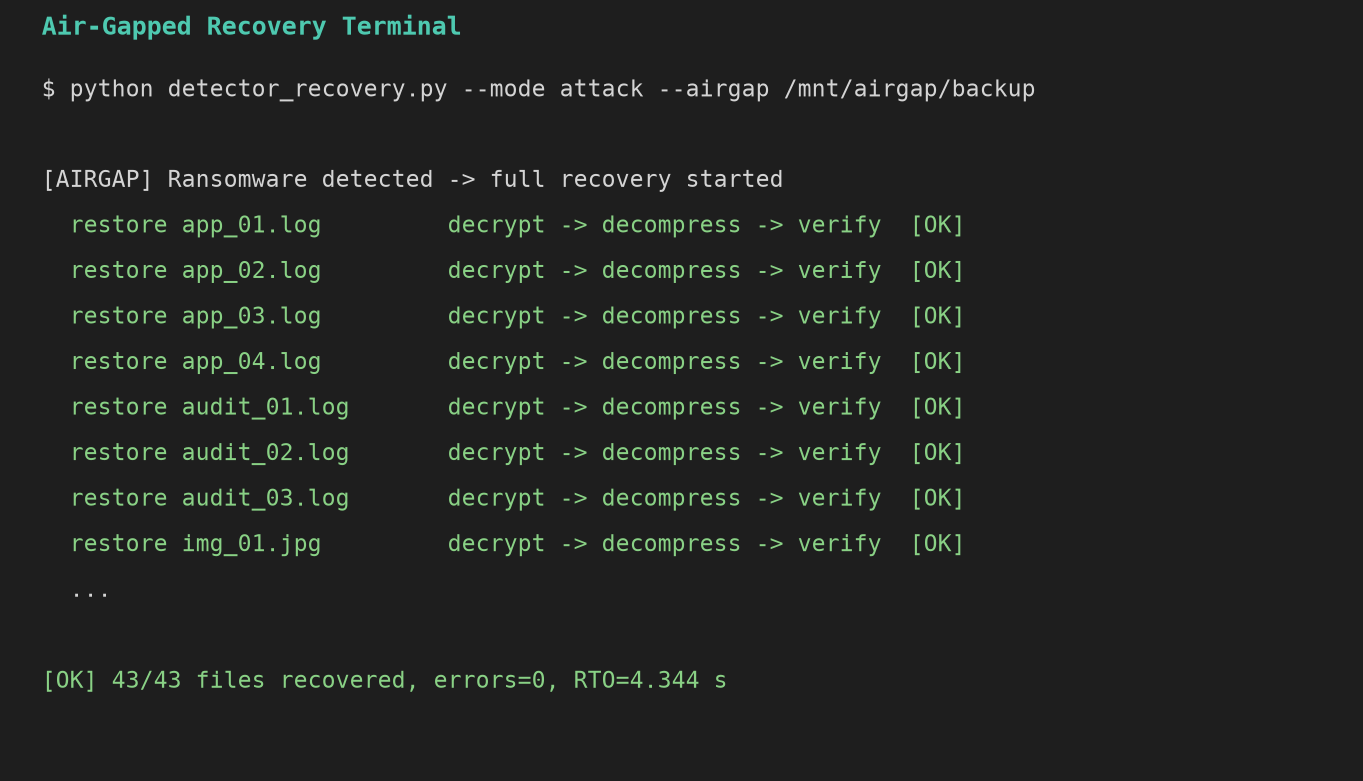
\includegraphics[width=0.6\textwidth]{figures/figure16_restore_terminal_en.png}
\vspace{.4em}
\caption{Air-gapped restore process terminal showing recovery and checksum validation of all files}
\label{fig:restore_terminal}
\end{figure}

Recovery is measured by RTO (time to recover all 43 files from \textit{air-gapped} storage after anomaly detection) on AWS EC2 with a $\approx490$~MB \textit{dataset} (Table~\ref{tab:rto}). Each scenario recovered 43/43 files without error.

\begin{table}[H]
\centering
\fontsize{8pt}{10pt}\selectfont
\caption{Measured Recovery Time Objective (RTO) for recovering all 43 files}
\label{tab:rto}
\begin{tabular}{l c c c}
\hline
\textbf{Attack Type} & \textbf{Total Files} & \textbf{Files Recovered} & \textbf{RTO (s)} \\
\hline
Encrypt-and-Hold (CVE-2017-0144)           & 43 & 43 & 4.34 \\
Metadata/Header Corruption (CVE-2018-8453) & 43 & 43 & 5.21 \\
Overwrite-and-Corrupt (CVE-2021-36934)     & 43 & 43 & 5.34 \\
\hline
\end{tabular}
\end{table}

RTO ranges 4.3--5.3~s for the whole test \textit{dataset}. Because the workflow is deterministic and grows about linearly with volume, RTO extrapolates proportionally for enterprise scale; full-scale validation (files up to 1~GB) is future work.

\subsection{Cross-platform consistency (Windows vs Linux)}
The same experiment ran on AWS EC2 Windows Server 2022 and Ubuntu 22.04 (Table~\ref{tab:cross_platform}). Compression ratios are practically identical (they depend on data and algorithm, not OS); only RTO differs slightly due to hardware. Detection and recovery are perfect on both (43/43, FPR/FNR 0\%).

\begin{table}[H]
\centering
\fontsize{8pt}{10pt}\selectfont
\caption{Consistency of results across two platforms (43 files)}
\label{tab:cross_platform}
\begin{tabular}{l c c}
\hline
\textbf{Metric} & \textbf{Windows Server 2022} & \textbf{Ubuntu 22.04} \\
\hline
Log/TXT saving (Brotli) & 89.6\% & 89.5\% \\
CSV saving (Brotli)     & 81.1\% & 81.1\% \\
JPG / XLSX saving       & $\approx$0\% & $\approx$0\% \\
Detection (all attacks) & 43/43 & 43/43 \\
Successful recovery     & 43/43 & 43/43 \\
FPR / FNR               & 0\% / 0\% & 0\% / 0\% \\
RTO Encrypt-and-Hold (s) & 5.50 & 4.34 \\
RTO Metadata Corruption (s) & 5.20 & 5.21 \\
RTO Overwrite-and-Corrupt (s) & 5.32 & 5.34 \\
\hline
\end{tabular}
\end{table}

This agreement confirms that adaptive compression, integrity verification, and \textit{air-gapped} recovery work reliably and reproducibly on both local Windows and \textit{cloud} Linux/Windows infrastructure, strengthening external validity.

\subsection{False positive and false negative evaluation}
To assess detection reliability, FPR and FNR were measured by comparing legitimate AES-256 backup encryption against simulated ransomware that modifies content and metadata; on detecting abnormal changes the system auto-activated \textit{air-gapped} recovery and replaced corrupted files from isolated copies (Table~\ref{tab:detection_accuracy}).

\begin{table}[H]
\centering
\fontsize{8pt}{10pt}\selectfont
\caption{Detection and recovery accuracy evaluation}
\label{tab:detection_accuracy}
\begin{tabularx}{\textwidth}{@{}X c c c c c@{}}
\hline
\textbf{Scenario} & \textbf{Total Files} & \textbf{Detected as Ransomware} & \textbf{Auto Air-Gapped Restore} & \textbf{Actual Status} & \textbf{Result} \\
\hline
Normal AES-256 backup encryption & 43 & 0 & No & Safe & True Negative \\
Encrypt and Hold attack & 43 & 43 & Yes & Ransomware & True Positive \\
Metadata/Header Corruption & 43 & 43 & Yes & Ransomware & True Positive \\
Overwrite and Corrupt & 43 & 43 & Yes & Ransomware & True Positive \\
\hline
\end{tabularx}
\end{table}

The results yield \textbf{FPR = 0\%} and \textbf{FNR = 0\%}: the system distinguishes legitimate AES-256 backup encryption from unauthorized ransomware modification, and on detecting anomalies auto-restores clean versions from \textit{air-gapped} backup.

It must be emphasized that these 0\% values are a \textbf{logical consequence} of \textit{hash}-integrity detection in a controlled environment, \textbf{not} a claim of perfect real-world detection. Because any modification---even a single \textit{byte}---deterministically changes the SHA-256 \textit{hash}, all simulated corruption is necessarily detected, while legitimate encryption is never falsely flagged since its baseline is recorded beforehand. Integrity-based mechanisms detect \textit{that} a file changed but not the \textit{behavior} of a process, so they remain vulnerable to sophisticated \textit{evasion} (FPE, \textit{fileless}, \textit{Living-off-the-Land}) not represented in this study's synthetic \textit{dataset}. These FPR/FNR figures should thus be read as functional validation of the mitigation/recovery stage, not as a benchmark of detection accuracy in general.

\subsection{Distinguishing normal encryption from ransomware}
In normal backup, the system records \textit{hash} and metadata as an integrity baseline after controlled encryption/compression. Ransomware simulation instead introduces significant deviations in \textit{hash} and structure that do not match the baseline, which the integrity validation detects, identifying compromised files. Combining \textit{hash} checking, metadata analysis, and \textit{air-gapped} backup effectively preserves integrity while enabling secure recovery during attacks.

\subsection{Security analysis of the logical air-gap and window of vulnerability}
Unlike a physical \textit{air-gap} that fully severs the connection, the logical \textit{air-gap} isolates the backup volume by \textit{mounting} it only during an active backup/recovery window. This is more affordable and practical, but honestly leaves a \textbf{window of vulnerability}: while mounted, the volume is technically reachable by other \textit{host} processes, and \textit{memory-resident} ransomware could wait for a \textit{mount} event to write a payload. Logical isolation therefore substantially reduces---but does not eliminate---the attack surface versus a continuously connected repository.

To narrow this window, recommended mitigations for deployment are: (i) strict IAM access control so only authorized backup processes may \textit{mount} and write; (ii) read-only \textit{mount} during recovery so restoration cannot be abused to write payloads; (iii) \textit{immutable}/WORM storage (e.g., \textit{object lock} on cloud object storage) so written versions cannot be altered/deleted during retention; and (iv) minimizing \textit{mount} duration to the backup transaction only. Together these make the logical \textit{air-gap} a reasonable balance of cost, operational ease, and resilience, and point toward a \textit{zero-trust backup} architecture in future work.

\section{Conclusion}
\label{sec:conclusion}
A cloud-based backup system integrating an \textit{air-gapped} mechanism with multi-algorithm \textit{lossless} compression was developed to improve ransomware resilience while optimizing storage. It performs compression, backup, anomaly detection, and automated recovery in one integrated environment. Compression performance depends on data characteristics: Snappy/LZ4 are faster for small-to-medium files, while Brotli/Zstandard achieve the highest ratios on low-entropy text (savings up to 89.5\% for logs and 81.1\% for CSV); already-compressed JPG/XLSX save near zero, matching the \textit{lossless} limit.

Controlled ransomware simulations (no real \textit{malware}) on a 43-file synthetic \textit{dataset}, using CVE-2017-0144, CVE-2018-8453, and CVE-2021-36934 patterns, showed the system preserved integrity and achieved 100\% recovery across all 43 files via the \textit{air-gapped} mechanism, with the anomaly detector flagging unauthorized modifications while keeping zero \textit{false positives} on legitimate AES-256 operations. Integrating \textit{air-gapped} backup with multi-algorithm compression thus significantly enhances both resilience and storage efficiency in cloud backup.

The adaptive mechanism uses rule-based selection for its low \textit{overhead}, lightweight implementation, and fast decisions---suited to financial cloud systems needing reliability and low-latency operation. Limitations open future directions: validation used a limited synthetic \textit{dataset} (43 files) via controlled simulation, so generalization to enterprise scale and real ransomware remains to be tested; and detection relies on \textit{hash}/metadata integrity, not yet handling sophisticated evasion. Promising directions: (i) evolving rule-based selection into \textit{machine learning} (e.g., \textit{Random Forest}) for larger, heterogeneous data; (ii) testing real ransomware in a safe \textit{sandbox}; (iii) integrating \textit{immutable}/WORM storage and \textit{zero-trust backup}; (iv) formal security analysis and stronger \textit{key management}; (v) enterprise-scale evaluation of \textit{throughput}, CPU/RAM, energy, and \textit{cloud} cost; and (vi) comparison with \textit{incremental backup} and \textit{deduplication}. These would further strengthen the credibility, resilience, and practical feasibility of the ransomware-resilient backup system.

\section*{FUNDING INFORMATION}
\label{sec:funding}
This research was supported by Politeknik Elektronika Negeri Surabaya and conducted in collaboration with PT Equnix Business Solution with support from internal resources.

\section*{AUTHOR CONTRIBUTIONS STATEMENT}
\label{sec:credit}
This study employs the Contributor Roles Taxonomy (CRediT) to acknowledge individual author contributions, mitigate authorship conflicts, and enhance collaboration.

\begin{table}[H]
	\centering
	\selectfont
	\begin{tabular}{lcccccccccccccc}
		\hline
		\textbf{Name of Author} & \cellcolor[HTML]{D8F0F8}\textbf{C} & \cellcolor[HTML]{D8F0F8}\textbf{M} & \textbf{So} & \textbf{Va} & \cellcolor[HTML]{D8F0F8}\textbf{Fo} & \cellcolor[HTML]{D8F0F8}\textbf{I} & \textbf{R} & \textbf{D} & \cellcolor[HTML]{FDE9D9}\textbf{O} & \cellcolor[HTML]{FDE9D9}\textbf{E} & \textbf{Vi} & \textbf{Su} & \textbf{P} & \textbf{Fu} \\
		\hline
		Hero Yudo Martono & \cellcolor[HTML]{D8F0F8}\checkmark & \cellcolor[HTML]{D8F0F8}\checkmark & \checkmark & \checkmark & \cellcolor[HTML]{D8F0F8}\checkmark & \cellcolor[HTML]{D8F0F8}\checkmark &  & \checkmark & \cellcolor[HTML]{FDE9D9}\checkmark & \cellcolor[HTML]{FDE9D9}\checkmark &  & \checkmark & \checkmark & \checkmark \\
		Nafisah Rahmadani H. & \cellcolor[HTML]{D8F0F8} & \cellcolor[HTML]{D8F0F8}\checkmark & \checkmark &  & \cellcolor[HTML]{D8F0F8}\checkmark & \cellcolor[HTML]{D8F0F8}\checkmark & \checkmark & \checkmark & \cellcolor[HTML]{FDE9D9}\checkmark & \cellcolor[HTML]{FDE9D9} & \checkmark &  &  &  \\
		Iwan Syarif & \cellcolor[HTML]{D8F0F8}\checkmark & \cellcolor[HTML]{D8F0F8}\checkmark &  & \checkmark & \cellcolor[HTML]{D8F0F8} & \cellcolor[HTML]{D8F0F8} &  &  & \cellcolor[HTML]{FDE9D9} & \cellcolor[HTML]{FDE9D9}\checkmark &  & \checkmark &  &  \\
		Ferry Astika Saputra & \cellcolor[HTML]{D8F0F8}\checkmark & \cellcolor[HTML]{D8F0F8}\checkmark &  & \checkmark & \cellcolor[HTML]{D8F0F8} & \cellcolor[HTML]{D8F0F8} &  &  & \cellcolor[HTML]{FDE9D9} & \cellcolor[HTML]{FDE9D9}\checkmark &  & \checkmark &  &  \\
		\hline
		\multicolumn{15}{c}{
			\begin{tabular}{llllll}
				&&&&&\\
				C &: 	\textbf{C}\fontsize{8}{10}\selectfont onceptualization \quad\quad\quad\quad\quad\quad& I &: 	\textbf{I}\fontsize{8}{10}\selectfont nvestigation & Vi&: 	\textbf{Vi}\fontsize{8}{10}\selectfont sualization  \\
				M &: 	\textbf{M}\fontsize{8}{10}\selectfont ethodology & R &: 	\textbf{R}\fontsize{8}{10}\selectfont esources & Su&: 	\textbf{Su}\fontsize{8}{10}\selectfont pervision  \\
				So&: 	\textbf{So}\fontsize{8}{10}\selectfont ftware & D &:	\textbf{D}\fontsize{8}{10}\selectfont ata Curation & P &: 	\textbf{P}\fontsize{8}{10}\selectfont roject Administration  \\
				Va&: 	\textbf{Va}\fontsize{8}{10}\selectfont lidation & O &:	\fontsize{8}{10}\selectfont Writing - \fontsize{10}{12}\selectfont \textbf{O}\fontsize{8}{10}\selectfont riginal Draft & Fu&: 	\textbf{Fu}\fontsize{8}{10}\selectfont nding Acquisition \\
				Fo&: 	\textbf{Fo}\fontsize{8}{10}\selectfont rmal Analysis & E &:	\fontsize{8}{10}\selectfont Writing - Review \& \fontsize{10}{12}\selectfont\textbf{E}\fontsize{8}{10}\selectfont diting \quad\quad\quad\quad\quad\quad&  \\
			\end{tabular}
		}
	\end{tabular}
\end{table}

\section*{CONFLICT OF INTEREST STATEMENT}
\label{sec:coi}
The authors declare that there is no conflict of interest regarding the publication of this paper.

\section*{DATA AVAILABILITY}
\label{sec:data}
Datasets used in this study were synthetically generated based on operational data characteristics and backup structures adapted from PT Equnix Business Solution environments. No real financial or confidential production data were used in this study.

\begin{thebibliography}{99}
\footnotesize
\itemsep 0pt

\bibitem{1} A. A. Majmuah, ``Survey on technique to prevent ransomware attack,'' \textsl{Bulletin of Informatics and Data Science}, vol. 1, no. 2, 2021.
\bibitem{2} K. Begovi\'c, M. Karabegovi\'c, and A. Huseinovi\'c, ``Cryptographic ransomware encryption detection: survey,'' \textsl{arXiv preprint arXiv:2306.12008}, 2023.
\bibitem{3} S. Mansfield-Devine, ``Ransomware: detection, prevention and cure,'' \textsl{Network Security}, vol. 2016, no. 9, pp. 5--8, 2016.
\bibitem{4} H. B. Pavlos, P. Nikolaos, A. Jawad, and J. William, ``Ransomware: analysing the impact on Windows Active Directory Domain Services,'' \textsl{Journal of Cyber Security Technology}, 2022.
\bibitem{5} M. Houria, O. Noura, and A. Abdelmalek, ``Ransomware: analysis of encrypted files,'' \textsl{International Journal of Information Security}, 2023.
\bibitem{6} G. Lu, Y. Liu, Y. Chen, C. Zhang, Y. Gao, and G. Zhong, ``A comprehensive detection approach of WannaCry: principles, rules and experiments,'' in \textsl{Proc. Int. Conf. Cyber-Enabled Distributed Computing and Knowledge Discovery (CyberC)}, 2020, pp. 41--49.
\bibitem{7} I. Athauda and H. Herath, ``Windows elevation of privilege serious SAM vulnerability (CVE-2021-36934),'' \textsl{Journal of Cybersecurity and Digital Forensics}, 2022.
\bibitem{8} A. Al-Fuqaha et al., ``A survey on ransomware trends and mitigation techniques,'' \textsl{Egyptian Informatics Journal}, vol. 21, no. 4, pp. 231--245, 2020.
\bibitem{9} Z. A. Syed and T. R. Soomro, ``Compression algorithms: Brotli, Gzip and Zopfli perspective,'' \textsl{International Journal of Computer Science and Network Security}, 2021.
\bibitem{10} F. A. Abdulazeez, I. T. Ahmed, and B. T. Hammad, ``Performance comparison of compression algorithms for large-scale log systems,'' \textsl{Journal of Computer \& Electrical Engineering Sciences}, 2024.
\bibitem{11} M. A. Rabbani, A. Budiyono, and A. Widjajarto, ``Implementasi dan analisis security auditing menggunakan open source software dengan framework MITRE ATT\&CK,'' \textsl{e-Proceeding of Engineering}, vol. 7, no. 2, 2020.
\bibitem{12} R. Y. Dwiaranda, A. Budiyono, and A. Widjajarto, ``Implementasi dan analisis security auditing menggunakan open source software dengan framework STRIDE,'' \textsl{e-Proceeding of Engineering}, vol. 7, no. 2, 2020.
\bibitem{13} M. Sahu and J. Panda, ``Performance evaluation of efficient hybrid compression methods for text using lossless algorithms,'' \textsl{arXiv preprint}, 2025.
\bibitem{14} H. Zhang et al., ``Optimized Snappy compression with enhanced encoding strategies,'' \textsl{Electronics}, 2024.
\bibitem{15} M. C. Ghanem, T. M. Chen, M. A. Ferrag, and M. E. Kettouche, ``ESASCF: automated security compliance framework,'' \textsl{arXiv preprint}, 2023.
\bibitem{16} S. Rouhani, R. Belchior, R. S. Cruz, and R. Deters, ``Distributed attribute-based access control system using a permissioned blockchain,'' \textsl{arXiv preprint}, 2020.
\bibitem{17} Y. Fauzi and R. A. Hamdan, ``Pendekatan metodologis dalam deteksi ancaman siber pada server hosting menggunakan NMAP dan Metasploit,'' \textsl{Jurnal SUDO}, 2024.
\bibitem{18} T. Ariyadi et al., ``Implementasi OWASP untuk analisis kerentanan dan keamanan sistem informasi,'' \textsl{Jurnal STORAGE}, 2023.
\bibitem{19} Sophos, ``The state of ransomware in financial services 2024,'' Sophos Ltd., 2024. [Online]. Available: https://www.sophos.com
\bibitem{20} R. Pal, M. Shaikh, J. Sagvekar, and P. Tiwari, ``Data resilience: secure emergency backup on cloud,'' \textsl{International Journal of Advanced Research in Science, Communication and Technology}, vol. 4, no. 7, 2024.
\bibitem{21} NIST, ``Security guidelines for storage infrastructure (SP 800-209),'' National Institute of Standards and Technology, 2024. [Online]. Available: https://nvlpubs.nist.gov
\bibitem{22} A. Nasif, Z. A. Othman, and N. S. Sani, ``The deep learning solutions on lossless compression methods for alleviating data load on IoT nodes in smart cities,'' \textsl{Sensors}, vol. 21, no. 12, p. 4223, 2021.
\bibitem{23} T. McIntosh, T. Susnjak, T. Liu, D. Xu, P. Watters, D. Liu, Y. Hao, A. Ng, and M. Halgamuge, ``Ransomware reloaded: re-examining its trend, research and mitigation in the era of data exfiltration,'' \textsl{ACM Computing Surveys}, vol. 57, no. 1, art. 18, pp. 1--40, 2024, doi: 10.1145/3691340.
\bibitem{24} S. Liu, F. Saeed, Z. Yang, and J. Chen, ``A comprehensive review on hyperspectral image lossless compression algorithms,'' \textsl{Remote Sensing}, vol. 17, no. 24, p. 3966, 2025.
\bibitem{25} J. Hua, H. Xu, Y. Du, and L. Du, ``Improved JPEG lossless compression for compression of intermediate layers in neural networks based on compute-in-memory,'' \textsl{Electronics}, vol. 13, no. 19, p. 3872, 2024.
\bibitem{26} C. Beaman, A. Barkworth, T. D. Akande, S. Hakak, and M. K. Khan, ``Ransomware: recent advances, analysis, challenges and future research directions,'' \textsl{Computers \& Security}, vol. 111, p. 102490, 2021, doi: 10.1016/j.cose.2021.102490.
\bibitem{27} M. Dawood et al., ``Cyberattacks and security of cloud computing: a complete guideline,'' \textsl{Symmetry}, vol. 15, no. 11, p. 1981, 2023.
\bibitem{28} A. Singh et al., ``Enhancing ransomware attack detection using transfer learning and deep learning ensemble models on cloud-encrypted data,'' \textsl{Electronics}, vol. 12, no. 18, p. 3899, 2023.
\bibitem{29} P. Novak et al., ``Multistage malware detection method for backup systems,'' \textsl{Technologies}, vol. 12, no. 2, p. 23, 2024.
\bibitem{30} Kritika, ``A comprehensive literature review on ransomware detection using deep learning,'' \textsl{Cyber Security and Applications}, vol. 3, p. 100078, 2025, doi: 10.1016/j.csa.2024.100078.
\bibitem{31} N. Ebrahimi Majd and T. Mazumdar, ``Ransomware classification using machine learning,'' in \textsl{Proc. 32nd Int. Conf. Advanced Information Networking and Applications (AINA)}, IEEE, 2023.
\bibitem{32} S. Enomoto, H. Kuzuno, H. Yamada, Y. Shiraishi, and M. Morii, ``Early mitigation of CPU-optimized ransomware using monitoring encryption instructions,'' \textsl{International Journal of Information Security}, vol. 23, pp. 3393--3413, 2024, doi: 10.1007/s10207-024-00892-2.
\bibitem{33} M. Lang, L. Connolly, P. Taylor, and P. J. Connert, ``The evolving menace of ransomware: a comparative analysis of pre-pandemic and mid-pandemic attacks,'' \textsl{Digital Threats: Research and Practice}, vol. 4, no. 4, pp. 1--22, 2023, doi: 10.1145/3558006.
\bibitem{34} Z. Pan and Z. Shu, ``Hardware-assisted ransomware detection using automated machine learning,'' in \textsl{Proc. Design, Automation \& Test in Europe Conf. (DATE)}, IEEE, 2025.
\bibitem{35} Y. Hou, L. Guo, C. Zhou, Y. Xu, Z. Yin, S. Li, C. Sun, and Y. Jiang, ``An empirical study of data disruption by ransomware attacks,'' in \textsl{Proc. IEEE/ACM 46th Int. Conf. Software Engineering (ICSE)}, 2024, pp. 1--12.
\bibitem{36} M. Smith and J. Lee, ``Performance evaluation of compression algorithms for cloud storage,'' \textsl{Data in Brief}, vol. 48, pp. 1--10, 2023.
\bibitem{37} S. Kumar and R. Patel, ``Optimization of cloud backup against ransomware attacks,'' \textsl{IEEE Access}, vol. 10, pp. 45821--45835, 2022.
\bibitem{38} A. Novak, P. Chen, and R. Singh, ``Hybrid compression and air-gapped backup for ransomware mitigation,'' in \textsl{Proc. USENIX Security Symposium}, 2021.
\bibitem{39} L. Zhao and T. Wang, ``Text compression optimization using hybrid algorithms,'' \textsl{arXiv preprint arXiv:2501.12345}, 2025.
\bibitem{40} P. H. Meland, Y. F. F. Bayoumy, and G. Sindre, ``The ransomware-as-a-service economy within the darknet,'' \textsl{Computers \& Security}, vol. 92, p. 101762, 2020, doi: 10.1016/j.cose.2020.101762.
\bibitem{41} G. Nagar, ``The evolution of ransomware: tactics, techniques, and mitigation strategies,'' \textsl{SSRN Electronic Journal}, 2024, doi: 10.2139/ssrn.4881213.
\bibitem{42} A. Kapoor, A. Gupta, R. Gupta, S. Tanwar, G. Sharma, and I. E. Davidson, ``Ransomware detection, avoidance, and mitigation scheme: a review and future directions,'' \textsl{Sustainability}, vol. 14, no. 1, p. 8, 2022, doi: 10.3390/su14010008.
\bibitem{43} J. Lee, J. Kim, H. Jeong, and K. Lee, ``A machine learning-based ransomware detection method for attackers' neutralization techniques using format-preserving encryption,'' \textsl{Sensors}, vol. 25, no. 8, p. 2406, 2025, doi: 10.3390/s25082406.
\bibitem{44} J. Thomas and G. Galligher, ``Improving backup system evaluations in information security risk assessments to combat ransomware,'' \textsl{Computer and Information Science}, vol. 11, no. 1, pp. 25--38, 2018, doi: 10.5539/cis.v11n1p25.
\bibitem{45} B. Bahl and R. Endicott, ``Know thy ransomware response: a detailed framework for devising effective ransomware response strategies,'' \textsl{Digital Threats: Research and Practice}, vol. 4, no. 4, pp. 1--19, 2020, doi: 10.1145/3560022.
\bibitem{46} P. Yan and T. T. Khoei, ``Securing the Internet of Things: a comprehensive review of ransomware attacks, detection, countermeasures, and future prospects,'' \textsl{Franklin Open}, vol. 11, art. 102056, 2025, doi: 10.1016/j.fraope.2025.102056.

\end{thebibliography}

\section*{BIOGRAPHIES OF AUTHORS}
\label{sec:biographies}

\noindent
\begin{tabularx}{\textwidth}{@{}m{2.5cm}@{\hspace{0.4cm}}X@{}}
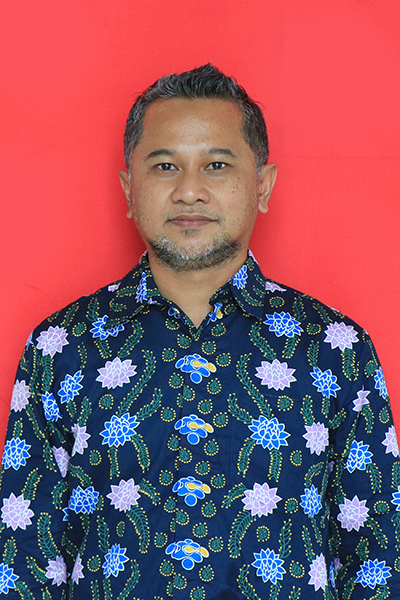
\includegraphics[width=2.5cm,height=3.2cm,keepaspectratio]{figures/hero_yudo.jpg} &
\textbf{Hero Yudo Martono} received his bachelor's degree in Computer Science (Electrical Engineering) from ITS, Indonesia. He then pursued a master's degree in Informatics Engineering from ITB, Indonesia. His research interests include cybersecurity, artificial intelligence, and cloud computing. He can be contacted at email: hero@pens.ac.id. \\
\end{tabularx}

\vspace{.7em}
\noindent
\begin{tabularx}{\textwidth}{@{}m{2.5cm}@{\hspace{0.4cm}}X@{}}
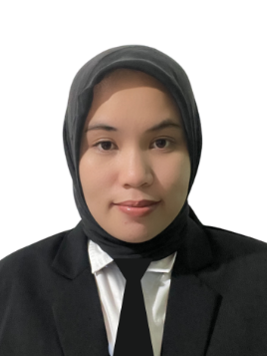
\includegraphics[width=2.5cm,height=3.2cm,keepaspectratio]{figures/nafisah.png} &
\textbf{Nafisah Rahmadani Harahap} is currently pursuing the Bachelor of Applied Engineering (D4) degree in Informatics Engineering at Politeknik Elektronika Negeri Surabaya (PENS), Indonesia. She is also working as an ERP Project Manager, focusing on enterprise resource planning implementation, business process optimization, project coordination, and digital transformation initiatives. Her research interests include cybersecurity, information systems, artificial intelligence, cloud computing, and enterprise software solutions. She can be contacted at email: nafisah@it.student.pens.ac.id. \\
\end{tabularx}

\vspace{.7em}
\noindent
\begin{tabularx}{\textwidth}{@{}m{2.5cm}@{\hspace{0.4cm}}X@{}}
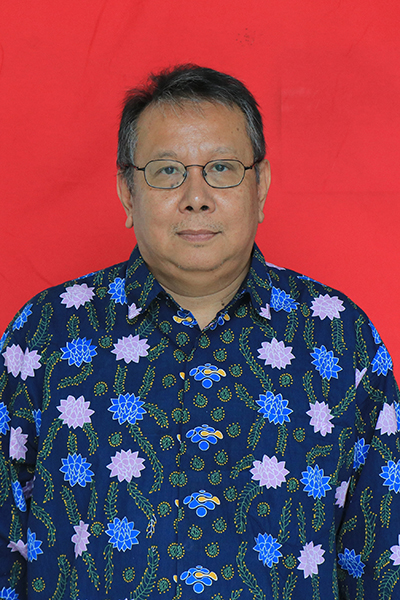
\includegraphics[width=2.5cm,height=3.2cm,keepaspectratio]{figures/iwan_syarif.jpg} &
\textbf{Iwan Syarif} is a professor (Ph.D.) and lecturer at the Department of Informatics Engineering, Politeknik Elektronika Negeri Surabaya (PENS), Indonesia. His research focuses on cybersecurity. He can be contacted at email: iwanarif@pens.ac.id. \\
\end{tabularx}

\vspace{.7em}
\noindent
\begin{tabularx}{\textwidth}{@{}m{2.5cm}@{\hspace{0.4cm}}X@{}}
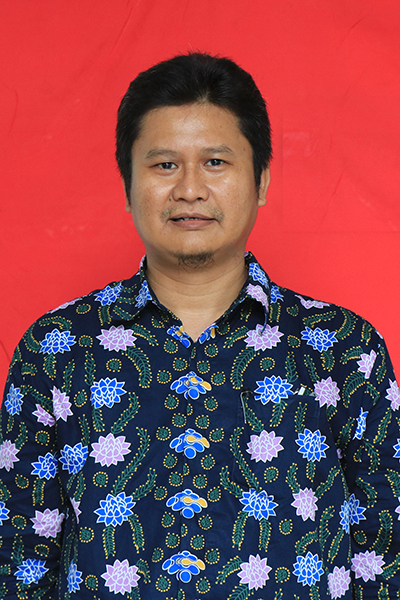
\includegraphics[width=2.5cm,height=3.2cm,keepaspectratio]{figures/ferry_astika.jpg} &
\textbf{Ferry Astika Saputra} received his doctoral (Ph.D.) degree from Universitas Indonesia and is a lecturer at the Department of Informatics Engineering, Politeknik Elektronika Negeri Surabaya (PENS), Indonesia. His research focuses on cybersecurity. He can be contacted at email: ferryas@pens.ac.id. \\
\end{tabularx}

\end{document}
